%% !TeX document-id = {4b9f5501-5408-4bec-8f26-68ce8212b968}
%% !TEX TS-program = pdflatexmk
%
%% To run: pdflatexmk + latex %

\title{Estimating population average treatment effects from experiments with noncompliance\thanks{The authors thank Jon McAuliffe and Jas Sekhon and his research group at UC Berkeley for valuable comments. Poulos acknowledges support from the National Science Foundation Graduate Research Fellowship [grant number DGE 1106400]. This work used the Extreme Science and Engineering Discovery Environment (XSEDE)-allocated systems Stampede2 at the Texas Advanced Computing Center (TACC) through allocation SES180010.}
}
\author{Kellie Ottoboni\thanks{Department of Statistics, University of California, Berkeley. email: \href{mailto:kellieotto@berkeley.edu}{\nolinkurl{kellieotto@berkeley.edu}}.} \hspace{10mm}
Jason Poulos\thanks{\emph{Corresponding author:} Department of Political Science, University of California, Berkeley. email: \href{mailto:poulos@berkeley.edu}{\nolinkurl{poulos@berkeley.edu}}.} 
\vspace{15mm}} 

\date{\today}

%%%%%%%%%%%%%%%%%%%%%%%%%%%%%%%%%%%%%%%%%%%%%%%%%%
% Set document class
\documentclass[hidelinks,12pt]{article}

% Define packages
\usepackage{graphicx,amsfonts,psfrag,layout,subcaption,array,longtable,lscape,booktabs,dcolumn,amsmath,amssymb,amssymb,amsthm,setspace,epigraph,chronology,color,xcolor,colortbl,wasysym}
\usepackage[]{graphicx}\usepackage[]{color}
\usepackage{enumitem}
\usepackage[page]{appendix}
\usepackage{hyperref, url} 
\usepackage[section]{placeins}
\usepackage[linewidth=1pt]{mdframed}
\usepackage[margin=1in]{geometry} %1 inch margins

% Footnotes stick at the bottom
\usepackage[bottom]{footmisc}

%Rm colons in empty captions
%\usepackage{caption}
%\captionsetup[figure]{labelformat=empty}

% New footnote characters
%\usepackage{footmisc}
%\DefineFNsymbols{mySymbols}{{\ensuremath\dagger}{\ensuremath\ddagger}\S\P
%   *{**}{\ensuremath{\dagger\dagger}}{\ensuremath{\ddagger\ddagger}}}
%\setfnsymbol{mySymbols}

% New tabular environment
\usepackage{tabularx}
\newcolumntype{Y}{>{\raggedleft\arraybackslash}X}% raggedleft column X

% Define appendix 
\renewcommand*\appendixpagename{Appendix}
\renewcommand*\appendixtocname{Appendix}

% Position floats
\renewcommand{\textfraction}{0.05}
\renewcommand{\topfraction}{0.95}
\renewcommand{\bottomfraction}{0.95}
\renewcommand{\floatpagefraction}{0.35}
\setcounter{totalnumber}{5}

% Colors for highlighting tables
\definecolor{Gray}{gray}{0.9}

% Different font in captions
%\newcommand{\captionfonts}{\scriptsize}
%
%\makeatletter  % Allow the use of @ in command names
%\long\def\@makecaption#1#2{%
%  \vskip\abovecaptionskip
%  \sbox\@tempboxa{{\captionfonts #1: #2}}%
%  \ifdim \wd\@tempboxa >\hsize
%    {\captionfonts #1: #2\par}
%  \else
%    \hbox to\hsize{\hfil\box\@tempboxa\hfil}%
%  \fi
%  \vskip\belowcaptionskip}
%\makeatother   % Cancel the effect of \makeatletter
 
% Set Spacing
\doublespacing

%Theorem
\newtheorem{theorem}{Theorem}

% Number assumptions
\newtheorem*{assumption*}{\assumptionnumber}
\providecommand{\assumptionnumber}{}
\makeatletter
\newenvironment{assumption}[2]
 {%
  \renewcommand{\assumptionnumber}{Assumption #1}%
  \begin{assumption*}%
  \protected@edef\@currentlabel{#1}%
 }
 {%
  \end{assumption*}
 }
\makeatother

% Macros
\newcommand{\Adv}{{\mathbf{Adv}}}       
\newcommand{\prp}{{\mathrm{prp}}}                  % How to define new commands 
\newcommand{\calK}{{\cal K}}
\newcommand{\outputs}{{\Rightarrow}}                
\newcommand{\getsr}{{\:\stackrel{{\scriptscriptstyle\hspace{0.2em}\$}}{\leftarrow}\:}}
\newcommand{\andthen}{{\::\;\;}}    %  \: \; for thinspace, medspace, thickspace
\newcommand{\Rand}[1]{{\mathrm{Rand}[{#1}]}}       % A command with one argument
\newcommand{\Perm}[1]{{\mathrm{Perm}[{#1}]}}       
\newcommand{\Randd}[2]{{\mathrm{Rand}[{#1},{#2}]}} % and with two arguments
\newcommand{\E}{\mathrm{E}}
\newcommand{\ind}{\mathbb{I}} % Indicator function
\newcommand{\pr}{\mathbb{P}} % Generic probability
\newcommand{\ex}{\mathbb{E}} % Generic expectation
\newcommand{\Var}{\mathrm{Var}}
\newcommand{\Cov}{\mathrm{Cov}}
\newcommand{\cov}{\mathrm{Cov}}
\DeclareMathOperator*{\plim}{plim}
\newcommand\independent{\protect\mathpalette{\protect\independenT}{\perp}}
\def\independenT#1#2{\mathrel{\rlap{$#1#2$}\mkern2mu{#1#2}}}
\newcommand{\possessivecite}[1]{\citeauthor{#1}'s [\citeyear{#1}]} 
\newcommand{\todo}[1]{{\color{red}{TO DO: \sc #1}}}

% Chicago 15 ed. author-date
\usepackage[utf8]{inputenc}
\usepackage[american]{babel}
\usepackage{csquotes}
\usepackage[authordate,backend=biber,natbib]{biblatex-chicago}
\addbibresource{refs.bib}

\begin{document}
\begin{singlespace} % single space for title
\maketitle  

\thispagestyle{empty}
\begin{abstract}  
\noindent 
This paper {\color{red} improves on the transportability of clinical trial results to a population by extending a method of estimating population average treatment effects in settings with noncompliance.} We identify the complier-average causal effect for {\color{red}a} target population with few additional assumptions. Simulations show the compliance-adjusted estimator performs better than the unadjusted estimator when compliance is relatively low and can be predicted by observed covariates. We apply the proposed estimator to measure the effect of Medicaid coverage on health care use for a target population of adults who may benefit from expansions to the Medicaid program{\color{red}, using} data from a large-scale health insurance experiment in which a small subset of those randomly selected to receive Medicaid benefits actually enrolled.
\end{abstract}	

\end{singlespace}
%Move introduction to second page
\pagebreak
\setcounter{page}{1} % Reset to Page 1

\vspace{20mm}

\section{Introduction}\label{intro}
Randomized control trials (RCTs) are the gold standard for estimating the causal effect of a treatment. An RCT may give an unbiased estimate of the sample average treatment effect (SATE), but external validity is an issue when the individuals in the RCT are unrepresentative of the actual population of interest. For example, the participants in an RCT in which individuals volunteer to sign up for health insurance may be in poorer health at baseline than the overall population. External validity is particularly relevant to policymakers who want to know how the SATE would generalize to the broader population. 

{\color{red}This paper extends the literature on extrapolating clinical trial results to populations to deal with noncompliance. Previous approaches to the problem of extrapolating RCT results to a population \citep{ImaKinStu08, stuart2011use, Hartman} are designed for settings where there is full compliance with treatment. This paper contributes to the literature by defining the assumptions required to identify complier--average causal effects for the target population and proposing a procedure to recover this estimand.} 

\citet{Hartman} propose a method of reweighting the responses of individuals in an RCT according to the distribution of covariates in the target population in order to estimate the population average treatment effect on the treated (PATT). Under a series of assumptions, the PATT is identified from the RCT outcomes. {\color{red}We extend the method to estimate the complier--average causal effects for the target population from RCT data with noncompliance.} Noncompliance, which occurs when individuals who are assigned to the treatment group do not comply with the treatment, is a prevalent issue in RCTs. It dilutes the estimated effect of treatment assignment, and the resulting intention--to--treat (ITT) estimate is biased towards zero.

The proposed estimator involves estimating the expectation of the response of compliers in the RCT sample, conditional on their covariates, where the expectation is taken over the distribution of population covariates. {\color{red}Note that our estimation strategy differs from reweighting methods that use propensity scores to adjust the RCT data \citep{stuart2011use}. In this context, the propensity score model predicts participation in the RCT, given pretreatment covariates common to both the RCT and population data. Individuals in the RCT and population are then weighted according to the inverse of the estimated propensity score. We use an ensemble of algorithms to predict the response surface for RCT compliers and use the predicted values from the response surface model to estimate the potential outcomes of population members who received treatment, given their covariates.

When estimating the average causal effect from an RCT, researchers typically divide the ITT estimate by the compliance rate under the identifying assumptions outlined in \citet{Angrist1996}. When extrapolating RCT results to a population, one might simply weight the PATT estimate by the population compliance rate in order to yield a population average effect of treatment on treated compliers.\footnote{A similar approach is used by \cite{imai2013experimental} for estimating average complier indirect effects.} However, the compliance rate is likely to differ between the sample and population, as well as across subgroups. We propose an alternative approach of actually identifying the likely compliers in the control group. By explicitly modeling compliance, our approach allows researchers to decompose population estimates by covariate group and also predict which population members are likely to comply with treatment. Both of these features are useful for policymakers in evaluating the efficacy of policy interventions for subgroups of interest in a population. 
}

We apply the proposed estimator to measure the effect of Medicaid coverage on health care use for a target population of adults who may benefit from government-backed expansions to the Medicaid program. We draw RCT data from a large-scale health insurance experiment, in which only $30\%$ of those randomly selected to receive Medicaid benefits actually enrolled. We find substantial differences between sample and population estimates in terms of race, education, and health status subgroups. 

The paper proceeds as follows: Section \ref{estimator} presents the proposed estimator, necessary assumptions for its identifiability, and an estimation procedure; Section \ref{sim} reports the estimator's performance in simulations; Section \ref{application} uses the estimator to identify the effect of extending Medicaid coverage to the low--income adult population in the U.S; Section \ref{discussion} discusses the results. 

\section{Estimator} \label{estimator}
We are interested in using the outcomes from an RCT to estimate the average treatment effect on the treated for a target population. Treatment in the population is not assigned at random, but rather may depend on other variables, confounding the effect of treatment on the outcome of interest. RCTs are needed to isolate the effect of treatment. However, strict exclusion criteria for RCTs often result in a sample whose distribution of covariates differs substantially from the target population. 

Ideally, we would take the results of an RCT and reweight the sample such that the reweighted covariates match the those in the population. In practice, one rarely knows the true covariate distribution in the target population. Instead, we consider data from a nonrandomized, observational study in which participants are representative of the target population. Our proposed estimator combines RCT and observational data to overcome these issues.

\subsection{Assumptions} \label{assumptions}
Let $Y_{ist}$ be the potential outcome for individual $i$ in group $s$, where $s=0$ is the population and $s=1$ is the RCT, and let $t$ be the treatment received. For simplicity, we assume there are only two possible treatments: $t=1$ for the active treatment and $t=0$ for the control or no treatment. Let $S_i$ denote the sample assignment, $T_i$ denote the treatment assigned, and $D_i$ denote treatment received. Let $W_i$ be individual $i$'s observable pretreatment covariates that are related to the sample selection mechanism for membership in the RCT, treatment assignment in the population, and complier status. Let $C_i$ be an indicator for individual $i$'s compliance to treatment{\color{red}, which is only observable in the RCT}. Treatment is assigned at random by the investigator in the RCT, so we observe both $D_i$ and $T_i$ when $S_i = 1$. For compliers in the RCT, $D_i = T_i$.

In the population, we suppose that treatment is made available to individuals based on their covariates $W_i$. Individuals with $T_i = 0$ do not receive treatment, while those with $T_i=1$ may decide whether or not to accept treatment. {\color{red}For individuals in the population, we only observe $D_i$ --- not $T_i$. We frame the Assumptions \ref{si_treat} and \ref{si_ctrl} defined below in terms of $C_i$ and $T_i$ in order to distinguish among the population controls noncompliers who should have received treatment (i.e., individuals with $T_i = 1$ and $D_i = 0$) from noncompliers assigned to control (i.e., individuals with $T_i = 1$ and $D_i = 0$). Differentiating population controls is important for deriving the estimator for $\tau_{\text{PATT}}$.

Assumptions \ref{consistency}, \ref{si_treat}, \ref{si_ctrl}, and \ref{sutva} are made by \citet{Hartman} to identify PATT from an RCT:
}

\vskip 0.2in
\begin{assumption}{1}{}\label{consistency}
	Consistency under parallel studies:
	\begin{equation*}
	Y_{i0t} = Y_{i1t}{\color{red}, \qquad \forall \, i \, , \, t=\{0,1\}.}
	\end{equation*}
\end{assumption} 

\noindent Assumption \ref{consistency} requires that each individual $i$ has the same response to treatments, whether $i$ is in the RCT or not. {\color{red} Compliance status $C_i$ is not a factor in this assumption because we assume that compliance is independent of sample and treatment assignment for all individuals with covariates $W_i$. 
	
\vskip 0.2in
\begin{assumption}{2}{}\label{compl}
	Conditional independence of compliance and assignment:
	\begin{equation*}
	C_i \independent {\color{red}S_i,\,T_i} \mid W_i, \qquad 0 < \pr(C_i = 1 \mid W_i) < 1. 
	\end{equation*}
\end{assumption}

\noindent Together, Assumptions \ref{consistency} and \ref{compl} ensure that potential outcomes do not differ based on sample assignment or receipt of treatment.}

\vskip 0.2in
\begin{assumption}{3}{}\label{si_treat}
	Strong ignorability of sample assignment for treated:
	\begin{equation*}
		(Y_{i01}, Y_{i11}) \independent S_i \mid (W_i, T_i=1,C_i=1), \qquad 0 < \pr(S_i=1 \mid W_i, T_i=1,C_i=1) <1.
	\end{equation*}
\end{assumption}

\noindent Assumption \ref{si_treat} ensures the potential outcomes for treatment are independent of sample assignment for individuals with the same covariates $W_i$ and assignment to treatment.\footnote{Throughout, we assume individuals are sampled randomly from an infinite population.} We make a similar assumption for the potential outcomes under control: 

\vskip 0.2in
\begin{assumption}{4}{}\label{si_ctrl}
	Strong ignorability of sample assignment for controls:
	\begin{equation*}
		(Y_{i00}, Y_{i10}) \independent S_i \mid (W_i, T_i=1,C_i= 1), \qquad 0 < \pr(S_i=1 \mid W_i, T_i=1,C_i=1) <1. 
\end{equation*}\end{assumption}

\color{red}

\noindent{\color{red} RCT study designs that apply restrictive exclusion criteria may increase the likelihood that there are unobserved differences between the RCT and target population, which would violate the strong ignorability assumptions.\footnote{Note that Assumptions \ref{si_treat} and \ref{si_treat} also imply strong ignorability of sample assignment for treated and control non-compliers since we assume in that compliance is also independent of sample and treatment assignment, conditional on $W_i$ (Assumption \ref{compl}). However, we are interested only on modeling the response surfaces for compliers.\label{ignorability-noncompliers}}

Interference undermines the framework because it creates more than two potential outcomes per participant, depending on the  treatment assignment of other participants \citep{rubin1990}. We therefore assume no interference between units: 

\vskip 0.2in
\begin{assumption}{5}{}\label{sutva}
	The potential outcomes $Y_{ist}$ do not depend on $T_j$, $\forall j\neq i$. 
	%\begin{equation*}
	%Y_{ist}^{L_i} = Y_{ist}^{L_j},  \forall i \neq j
	
	%\end{equation*}
	%where $L_j$ is the treatment and sample assignment vector for unit $j$. 
\end{assumption} 
\color{black}

Figure~\ref{fig:DAG} shows Assumptions \ref{si_treat}, \ref{si_ctrl}, and \ref{compl} in a directed acyclic graph. Treatment assignment $T_i$ may only depend on $C_i$ through $W_i$, and the potential outcomes $(Y_{is0}, Y_{is1})$ may only depend on $S_i$ through $W_i$. {\color{red}From the internal validity standpoint, the role of $W_i$ is critical: if any relevant observed covariates are not controlled, then there is a backdoor pathway from $T_i$ back to $W_i$ and into $Y_{ist}$. We use the same $W_i$ across all identifying assumptions, which implicitly assumes that the observable covariates that determine sample selection also determine population treatment assignment and complier status. This choice reflects a modeling assumption of our estimation procedure described in Section \ref{estimation}.}

%
%\vspace{10mm}
%\begin{center}
%[FIGURE 1 HERE]
%\end{center}

\begin{figure}[htbp]
\begin{center}
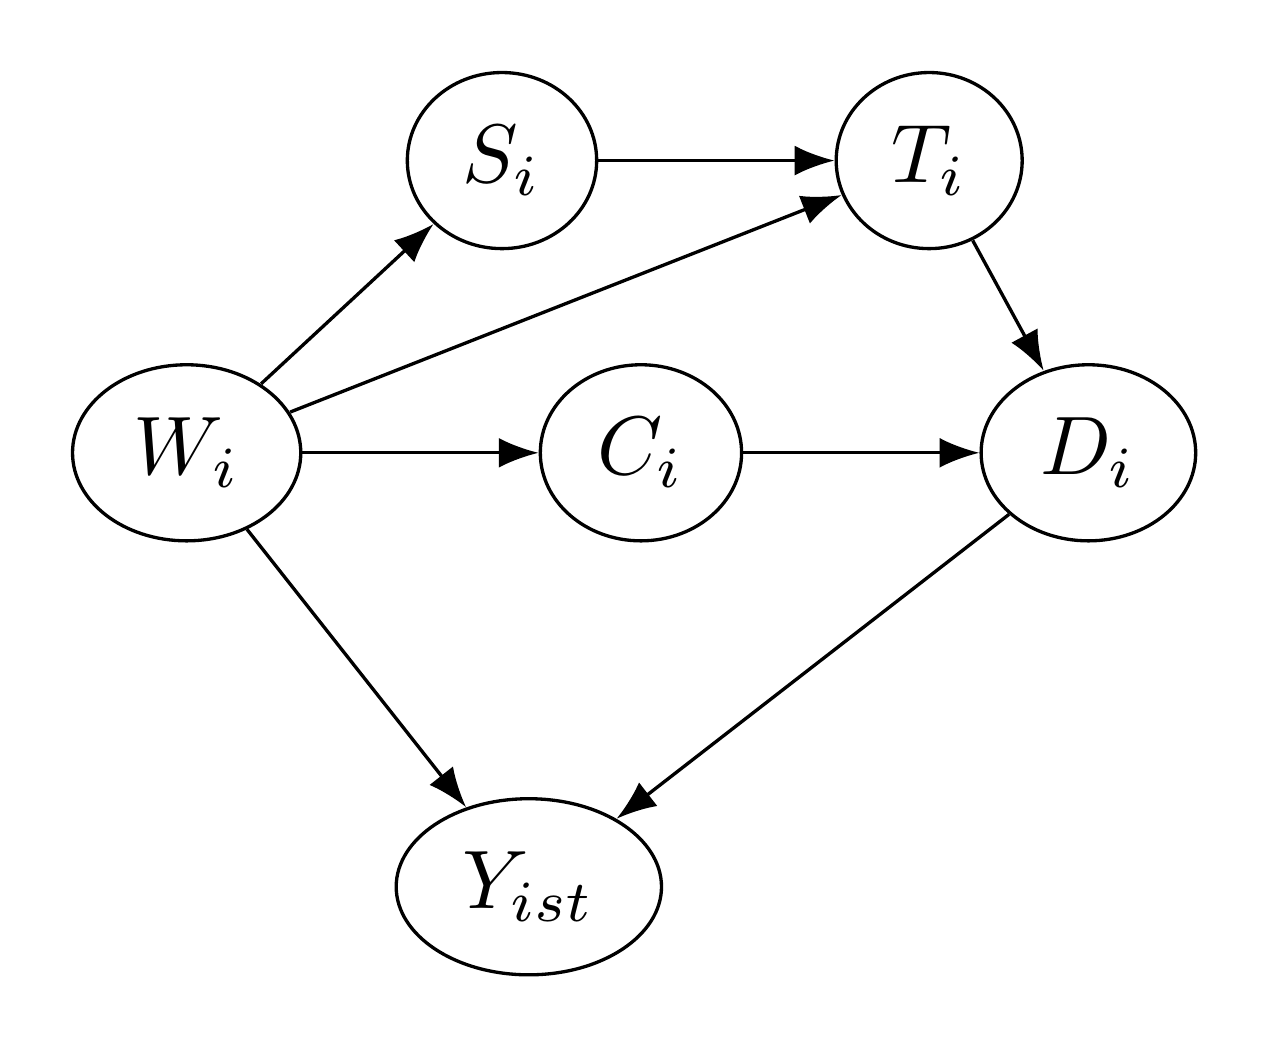
\includegraphics[width = 0.5\textwidth]{DAG2}
\caption{Causal diagram indicating the conditional independence assumptions needed to estimate the PATT-C.\label{fig:DAG}}
%\caption{\label{fig:DAG}}
\end{center}
\end{figure}

We additionally include Assumptions \ref{monotonicity} and \ref{ER}, which are made by \citet{Angrist1996} to ensure identifiability. The former assumption ensures that crossover is only possible from treatment to control:

\vskip 0.2in
\begin{assumption}{6}{}\label{monotonicity}
No defiers: 
\begin{equation*}
T_i \geq D_i {\color{red}, \qquad \forall \, i \, , \, t=\{0,1\}.}
\end{equation*}
\end{assumption}

Assumption \ref{ER} ensures treatment assignment affects the response only through the treatment received. In particular, the treatment effect may only be nonzero for compliers.

\begin{assumption}{7}{}\label{ER}
Exclusion restriction: For noncompliers,
\begin{equation*}
Y_{i11} = Y_{i10}, {\color{red}, \qquad \forall \, i.}
\end{equation*}  
\end{assumption}

\subsection{PATT and PATT-C}
The estimand of interest is the average treatment effect on those in the population who receive treatment:

\vskip 0.2in
\begin{equation}\label{tpatt}
\tau_{\text{PATT}} = \ex\left( Y_{i01} - Y_{i00} \mid S_i=0, D_i=1\right),
\end{equation}
\vskip 0.2in

It includes individuals who actually receive the treatment, but does not include those who are eligible for treatment and do not accept it (i.e., noncompliers). The following theorem, which we modify from \citet{Hartman} to account for noncompliance, relates the treatment effect in the population to the treatment effect in the RCT. {\color{red}The result enables us to estimate the Population Average Treatment Effect on Treated Compliers (PATT-C):}

\vskip 0.2in
\begin{theorem}\label{thm1}
Under Assumptions \ref{consistency} -- \ref{ER},
\begin{equation}\label{tpatt-est}
\tau_{\text{PATT-C}} = \ex_{01}\left[  \ex\left(Y_{i11} \mid S_i=1, D_i=1, W_i\right)\right]
-\ex_{01}\left[  \ex\left(Y_{i10} \mid S_i=1, T_i=0, C_i=1, W_i\right) \right] 
\end{equation}

where $\ex_{01}\left[\ex(\cdot \mid\dots, W_i)\right]$ denotes the expectation with respect to the distribution of $W_i$ in the treated individuals in the target population. 
\end{theorem}

\begin{proof}
We separate the expectation linearly into two terms and consider each individually.
\begin{align*}
\ex\left(Y_{i01} \mid S_i=0,D_i=1\right) &= \ex\left(Y_{i11} \mid S_i=0, D_i=1\right) \tag*{by Assumption \ref{consistency}} \\
&= \ex\left(Y_{i11} \mid S_i=0, T_i=1, C_i=1\right) \tag*{by Assumption \ref{monotonicity}} \\
&= \ex_{01}\left[  \ex\left(Y_{i11} \mid S_i=0, T_i=1, C_i=1, W_i\right) \right] \\
&= \ex_{01}\left[  \ex\left(Y_{i11} \mid S_i=1, T_i=1, C_i=1, W_i\right) \right] \tag*{by Assumption \ref{si_treat}} \\
&= \ex_{01}\left[  \ex\left(Y_{i11} \mid S_i=1, D_i=1, W_i\right)\right]
\end{align*}

{\color{red}Intuitively, conditioning on $W_i$ makes sample selection ignorable under Assumption \ref{si_treat}. This is the critical connector between the third and fourth lines of the first expectation derivation.}
	
\begin{align*}
\ex\left(Y_{i00} \mid S_i=0, D_i=1\right) &= \ex\left(Y_{i10} \mid S_i=0, D_i=1\right) \tag*{by Assumption \ref{consistency}} \\
&= \ex\left(Y_{i10} \mid S_i=0, T_i=1, C_i=1\right) \tag*{by Assumption \ref{monotonicity}} \\
&= \ex_{01}\left[  \ex\left(Y_{i10} \mid S_i=1, T_i=1, C_i=1, W_i\right) \right] \tag*{by Assumption \ref{si_ctrl}} \\
&= \ex_{01}\left[  \ex\left(Y_{i10} \mid S_i=1, T_i=0, C_i=1, W_i\right) \right] \\
\end{align*}

The last line follows because of the randomization carried out in the RCT, which guarantees $Y_{i10} \independent T_i \mid (W_i, S_i=1)$. Finally, the result follows by plugging these two expressions into Eq.~\eqref{tpatt}.
\end{proof}

\section{Estimation procedure}\label{estimation}
There are two challenges in turning Theorem~\ref{thm1} into an estimator of $\tau_{\text{PATT-C}}$ in practice. First, we must estimate the inner expectation over potential outcomes of compliers in the RCT. In our empirical example, we use an ensemble of algorithms \citep{van2007} to estimate the response surface for compliers in the RCT, given their covariates. Thus, the first term in the expression for $\tau_{\text{PATT-C}}$ is estimated by the weighted average of points on the response surface, evaluated for each treated population member's potential outcome under treatment. The second term is estimated by the weighted average of points on the response surface, evaluated for each treated population member's potential outcome under control.

The second challenge is that we cannot observe which individuals are included in the estimation of the second term. In the RCT control group, $C_i$ is unobservable, as they always receive no treatment ($D_i=0$). We must estimate the second term of Eq.~\eqref{tpatt-est} by predicting who in the control group would be a complier, had they been assigned to treatment. {\color{red}An alternative approach, is to simply weight the PATT estimate by the population compliance rate in order to yield a population average effect of treatment on treated compliers. However, the compliance rate is likely to differ between the sample and population, as well as across subgroups. Explicitly modeling compliance allows us to decompose PATT-C estimates by subgroup according to covariates common to both RCT and observational datasets.}

The procedure for estimating $\tau_{\text{PATT-C}}$ using Theorem~\ref{thm1} is as follows:
\begin{enumerate}[label=\textbf{S.\arabic*},ref=S.\arabic*]
\item Using the group assigned to treatment in the RCT $(S_i=1, T_i=1)$, train a model {\color{red}(or an ensemble of models)} to predict {\color{red}the probability of compliance as a function of covariates $W_i$.} \label{compliance-model}
\item Using the model from \ref{compliance-model}, predict who in the RCT assigned to control \textit{would have} complied to treatment had they been assigned to the treatment group. {\color{red} Complier status $C_i$ assumes the value 1 for individuals with a probability greater than 50\%, and is otherwise 0.} \label{complier-predict}
\item {\color{red}For the observed compliers assigned to treatment and predicted compliers assigned to control, train a model to predict the response using $W_i$ and $T_i$,\footnote{Note that assigned and observed treatment are the same for these individuals.} which gives} $\ex(Y_{i1t} \mid S_i=1, C_i=1, T_i=t, W_i)$ for $t \in \{0,1\}$.\label{response-model}
\item For all individuals who received treatment in the population $(S_i=0, D_i=1)$, estimate their potential outcomes $Y_{i10}$ and $Y_{i11}$ using the model from \ref{response-model}. The mean counterfactual $Y_{i11}$ minus the mean counterfactual $Y_{i10}$ is the estimate of $\tau_{\text{PATT-C}}$.\label{response-predict}
\end{enumerate}

Assumptions \ref{si_treat} and \ref{si_ctrl} are particularly important for estimating $\tau_{\text{PATT-C}}$: the success of the proposed estimator hinges on the assumption that the response surface is the same for compliers in the RCT and target population. If this does not hold, then the potential outcomes $Y_{i10}$ and $Y_{i11}$ for target population individuals cannot be estimated using the model from \ref{response-model}.\footnote{{\color{red}Section \ref{verifying} discusses whether the strong ignorability assumptions are plausible in the empirical application.}}

{\color{red}
\subsection{Modeling assumptions}  \label{modeling-assumptions}
}
In addition to the identification assumptions, we require additional modeling assumptions for the estimation procedure. We assume that the $W_i$ that determine sample selection also determine population treatment assignment and complier status. As pointed out in Section \ref{assumptions}, we also require that $W_i$ is complete because if any relevant elements of $W_i$ are not controlled, then there is a backdoor pathway from $T_i$ back to $W_i$ and into $Y_{ist}$. Lastly, we assume that the compliance model is accurate in predicting compliance in the training sample of RCT participants assigned to treatment and also generalizable to RCT participants assigned to control (\ref{compliance-model} and \ref{complier-predict}). Section \ref{ensemble} below describes our method of evaluating the generalizability of the compliance model.

{\color{red}
\subsection{Ensemble method}  \label{ensemble}
}

In the empirical application, we use the weighted ensemble method described in \citet{van2007} for \ref{compliance-model} and \ref{response-model} of the estimation procedure. This ensemble method combines algorithms with a convex combination of weights based on minimizing cross-validated error. It is shown to control for overfitting and outperforms single algorithms selected by cross-validation \citep{polley2010super}. 

We choose a variety of candidate algorithms to construct the ensemble, with a preference towards algorithms that tend to outperform in supervised classification tasks. We also have a preference for algorithms that have a built-in variable selection property. The idea is that we input the same $W_i$ and each candidate algorithm selects the most important covariates for predicting compliance status or potential outcomes. We select four types of candidate algorithms: gradient boosting machine; regularized linear model (e.g., Lasso or ridge regression) \citep{tibshirani2012strong}; neural network with a single hidden layer; and random forests \citep{breiman2001}. Lasso regression is an attractive because it tends to shrink all but one of the coefficients of correlated covariates to zero. 

\section{Simulations} \label{sim}
\color{red}We conduct a simulation study to compare the performance of the PATT and PATT-C estimators. For comparison, we also estimate the Sample Average Treatment Effect on the Treated Compliers (SATT-C) by fitting the response curve for compliers in the RCT --- which we do in \ref{response-model} for estimating $\tau_{\text{PATT-C}}$ --- and then taking the mean difference in potential outcomes for treated compliers in the sample:
\begin{equation}\label{tsatt-est} 
\tau_{\text{SATT-C}} = \ex(Y_{i11} \mid S_i=1, C_i=1, T_i=1, W_i) - \ex(Y_{i10} \mid S_i=1, C_i=1, T_i=1, W_i).
\end{equation}
\color{black}
Our simulation is designed so that the effect of treatment is heterogeneous and depends on covariates which are different in the RCT and target population. The design satisfies the conditional independence assumptions in Figure~\ref{fig:DAG}.

\subsection{Simulation design}
{\color{red}In the simulation, RCT eligibility, complier status, and treatment assignment in the population depend on multivariate normal covariates $(W^{1}_i, W^{2}_i, W^{3}_i, W^{4}_i)$ with mean $(0.5, 1, -1, -1)$ and covariances $\cov(W^{1}_i, W^{2}_i) = \cov(W^{1}_i, W^{4}_i)= \cov(W^{2}_i, W^{4}_i) = \cov(W^{3}_i, W^{4}_i) = 1$ and $\cov(W^{1}_i, W^{3}_i) = \cov(W^{2}_i, W^{3}_i) = 0.5$.  The first three covariates are observed by the researcher and $W^{4}_i$ is unobserved. }

The  equation for selection into the RCT is
 \vskip 0.2in
 $$ S_i = \ind(e_2 + g_1W^{1}_i + g_2W^{2}_i + g_3W^{3}_i + {\color{red}e_4W^{4}_i} + R > 0),$$
 \vskip 0.2in
where $R$ is standard normal. The parameter $e_2$ varies the fraction of the population eligible for the RCT and {\color{red}$e_4$ varies the degree of confounding with sample selection.} We set the constants $g_1, g_2,$ and $g_3$ to be $0.5,$ $0.25,$ and $0.75$, respectively.

Complier status is determined by
\vskip 0.2in
$$C_i = \ind(e_3 + h_2W^{2}_i + h_3W^{3}_i + {\color{red}e_5W^{4}_i} + Q > 0),$$
\vskip 0.2in
where $Q$ is standard normal, $e_3$ varies the fraction of compliers in the population, and {\color{red}$e_5$ varies the degree of confounding with treatment assignment.} We set the constants $h_2$ and $h_3$ to $0.5$.

For individuals in the population ($S_i=0$), treatment is assigned by
 \vskip 0.2in
  $$T_i = \ind(e_1 + f_1W^{1}_i + f_2W^{2}_i + {\color{red}e_6W^{4}_i} + V > 0),$$
  \vskip 0.2in
where $V$ is standard normal. Varying $e_1$ changes the fraction eligible for treatment in the population and {\color{red}$e_6$ varies the degree of confounding with sample selection.} We set the constants $f_1$ and $f_2$ to $0.25$ and $0.75$, respectively. For individuals in the RCT ($S_1=1$), treatment assignment is a sample from a Bernoulli distribution with probability $p=0.5$.
We set treatment received $D_i$ according to $T_i$ and $C_i$: $D_i = T_i$ if $C_i=1$ and $D_i = 0$ if $C_i=0$.

Finally, the response is determined by 
\vskip 0.2in
$$Y_{ist} = a + bD + c_1W^{1}_i + c_2W^{2}_i + dU.$$
\vskip 0.2in
We assume that the treatment effect $b$ is heterogeneous depending on $W^{1}_i$: $b = 1$ if $W^{1}_i > 0.75$ and $b=-1$ if $W^{1}_i \leq 0.75$.  We set $a, c_1,$ and $d$ to $1$ and $c_2$ to $2$. $U$ is standard normal and $U, V, R, Q, (W^{1}_i, W^{2}_i, W^{3}_i, W^{4}_i)$ are mutually independent.
 
We generate a population of 30,000 individuals and randomly sample 5,000. Those among the 5,000 who are eligible for the RCT ($S_i=1$) are selected. Similarly, we sample 5,000 individuals from the population and select those who are not eligible for the RCT ($S_i=0$): these are our observational study participants. This set-up mimics the reality that a population census is usually impossible.

We set each individual's treatment received $D_i$ according to their treatment assignment and complier status and observe their responses $Y_{ist}$. In this design, the way that we've set $S_i$, $T_i$, $D_i$, $C_i$, and $Y_{ist}$ ensures that Assumptions \ref{consistency} -- \ref{ER} hold.

{\color{red}
In the assigned-treatment RCT group $(S_i = 1, T_i = 1)$, we train a Gradient Boosting Machine (GBM) \citep{friedman2001greedy, friedman2002stochastic} on the covariates to predict who in the control group $(S_i = 1, T_i = 0)$ has $C_i=1$, which is unobservable.} These individuals \textit{would have} complied had they been assigned to the treatment group. For this group of observed compliers to treatment and predicted compliers from the control group of the RCT, we estimate the response surface {\color{red}using a GBM} with features $(W^{1}_i, W^{2}_i, W^{3}_i)$ and $D_i$. The PATT-C is estimated according to the estimation procedure outlined above.

\subsection{Simulation results}\label{sim-results}

{\color{red}We vary each of the parameters $e_1, e_2,$, $e_3$, $e_4$, $e_5$, and $e_6$ along a grid by $-2$ to $2$ in increments of $0.5$ in order to generate different combinations of rates of compliance, treatment eligibility, RCT eligibility in the population, and confounding in sample selection, treatment assignment, and compliance. For each possible combination of the six parameters, we run the simulation 10 times and compute the average root mean squared error (RMSE) of PATT-C, PATT, and the SATT-C.} All other parameters are held constant. The PATT and PATT-C estimates are obtained by estimating the response surface on all individuals in the RCT and applying \ref{response-predict} of our estimation procedure to the nonrandomized trial individuals. {\color{red}SATT-C is estimated using the predicted values from the response model trained in \ref{response-model}.}

Figure~\ref{fig:rmse_ratec_rates} shows the relationship between the percent of compliers in the whole population, the percentage of people in the whole population eligible to participate in the RCT, and the RMSE of the PATT and PATT-C estimators. The pattern of performance is qualitatively similar: both perform best when compliance is high and perform badly when compliance is low. {\color{red}Figure~\ref{fig:rmse_ratec_ratet}} shows that for a fixed rate of compliance, the RMSE of both estimators increases with the fraction of the total population eligible to participate in the RCT. When less than 70\% of the RCT is compliers, PATT-C tends to have lower RMSE than PATT.
%
%\vspace{10mm}
%\begin{center}
%[FIGURE 2 HERE]
%\end{center}

\begin{figure}[htbp]
\begin{center}
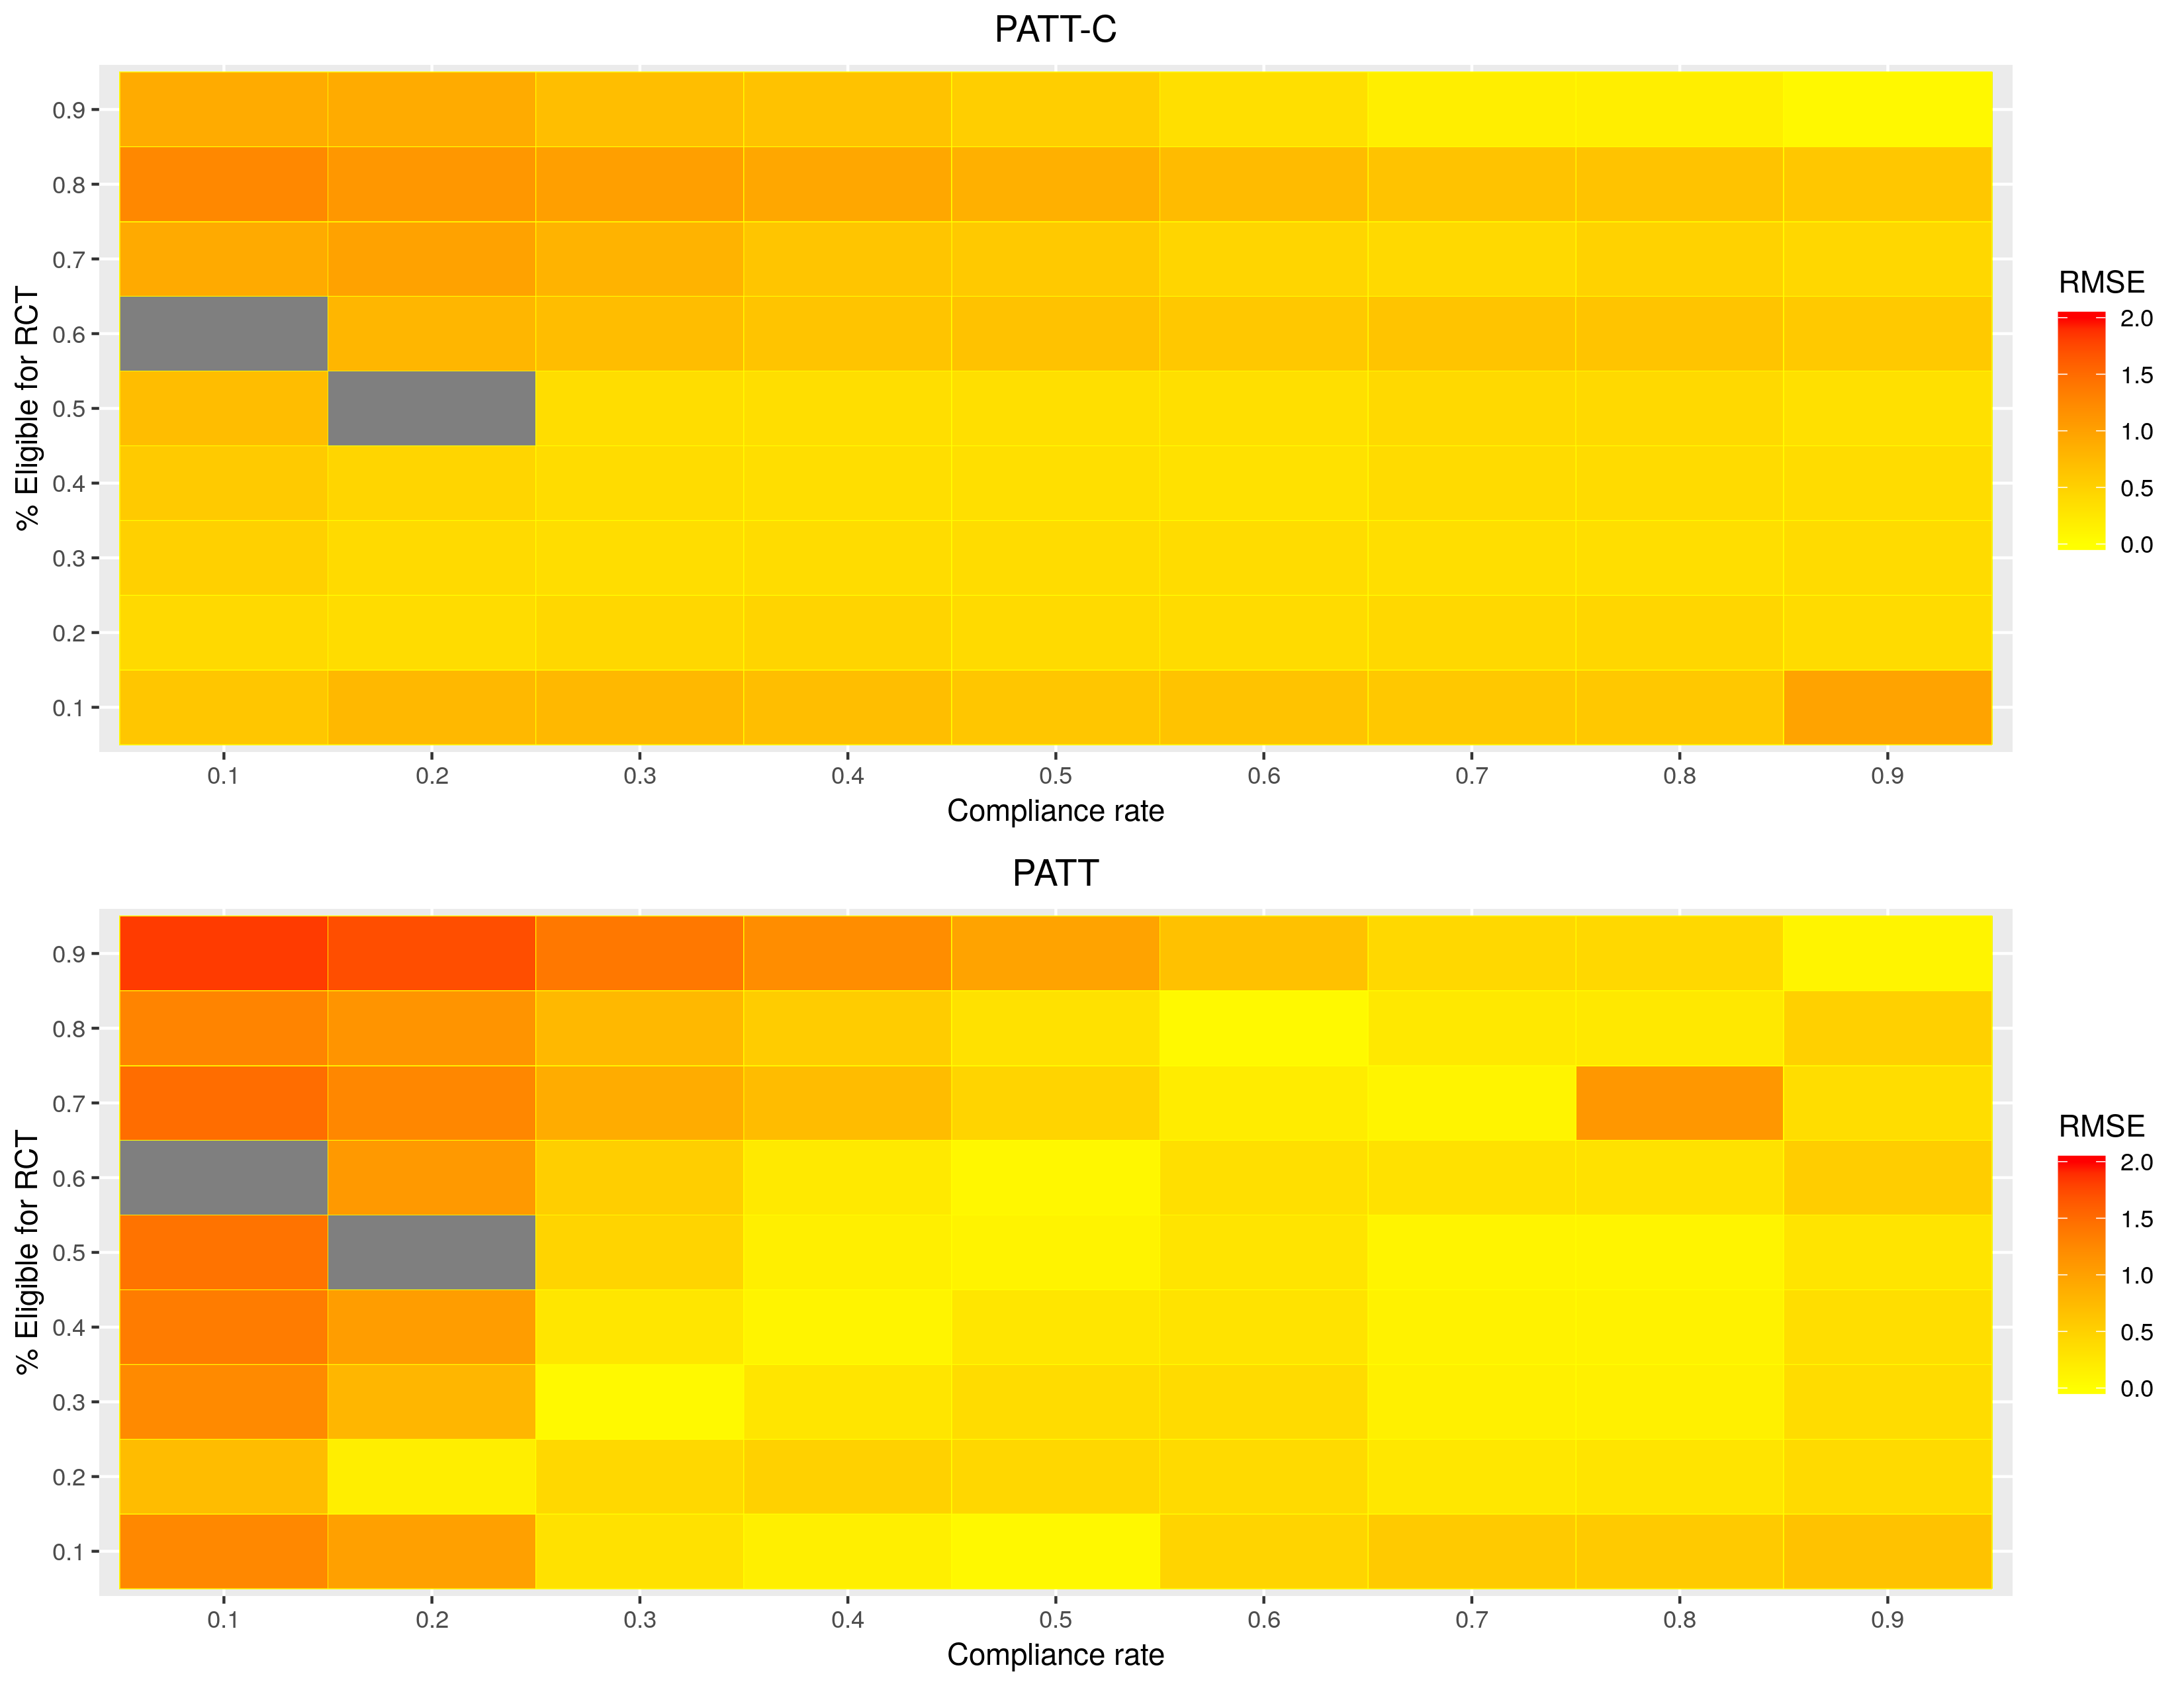
\includegraphics[width = 1\textwidth]{rmse_ratec_rates}
\caption{Simulated RMSE, binned by compliance rate and percent eligible for the RCT. Darker tiles correspond to higher RMSE.\label{fig:rmse_ratec_rates}}
%\caption{\label{fig:rmse_ratec_rates}}
\end{center}
\end{figure}

\begin{figure}[htbp]
	\begin{center}
		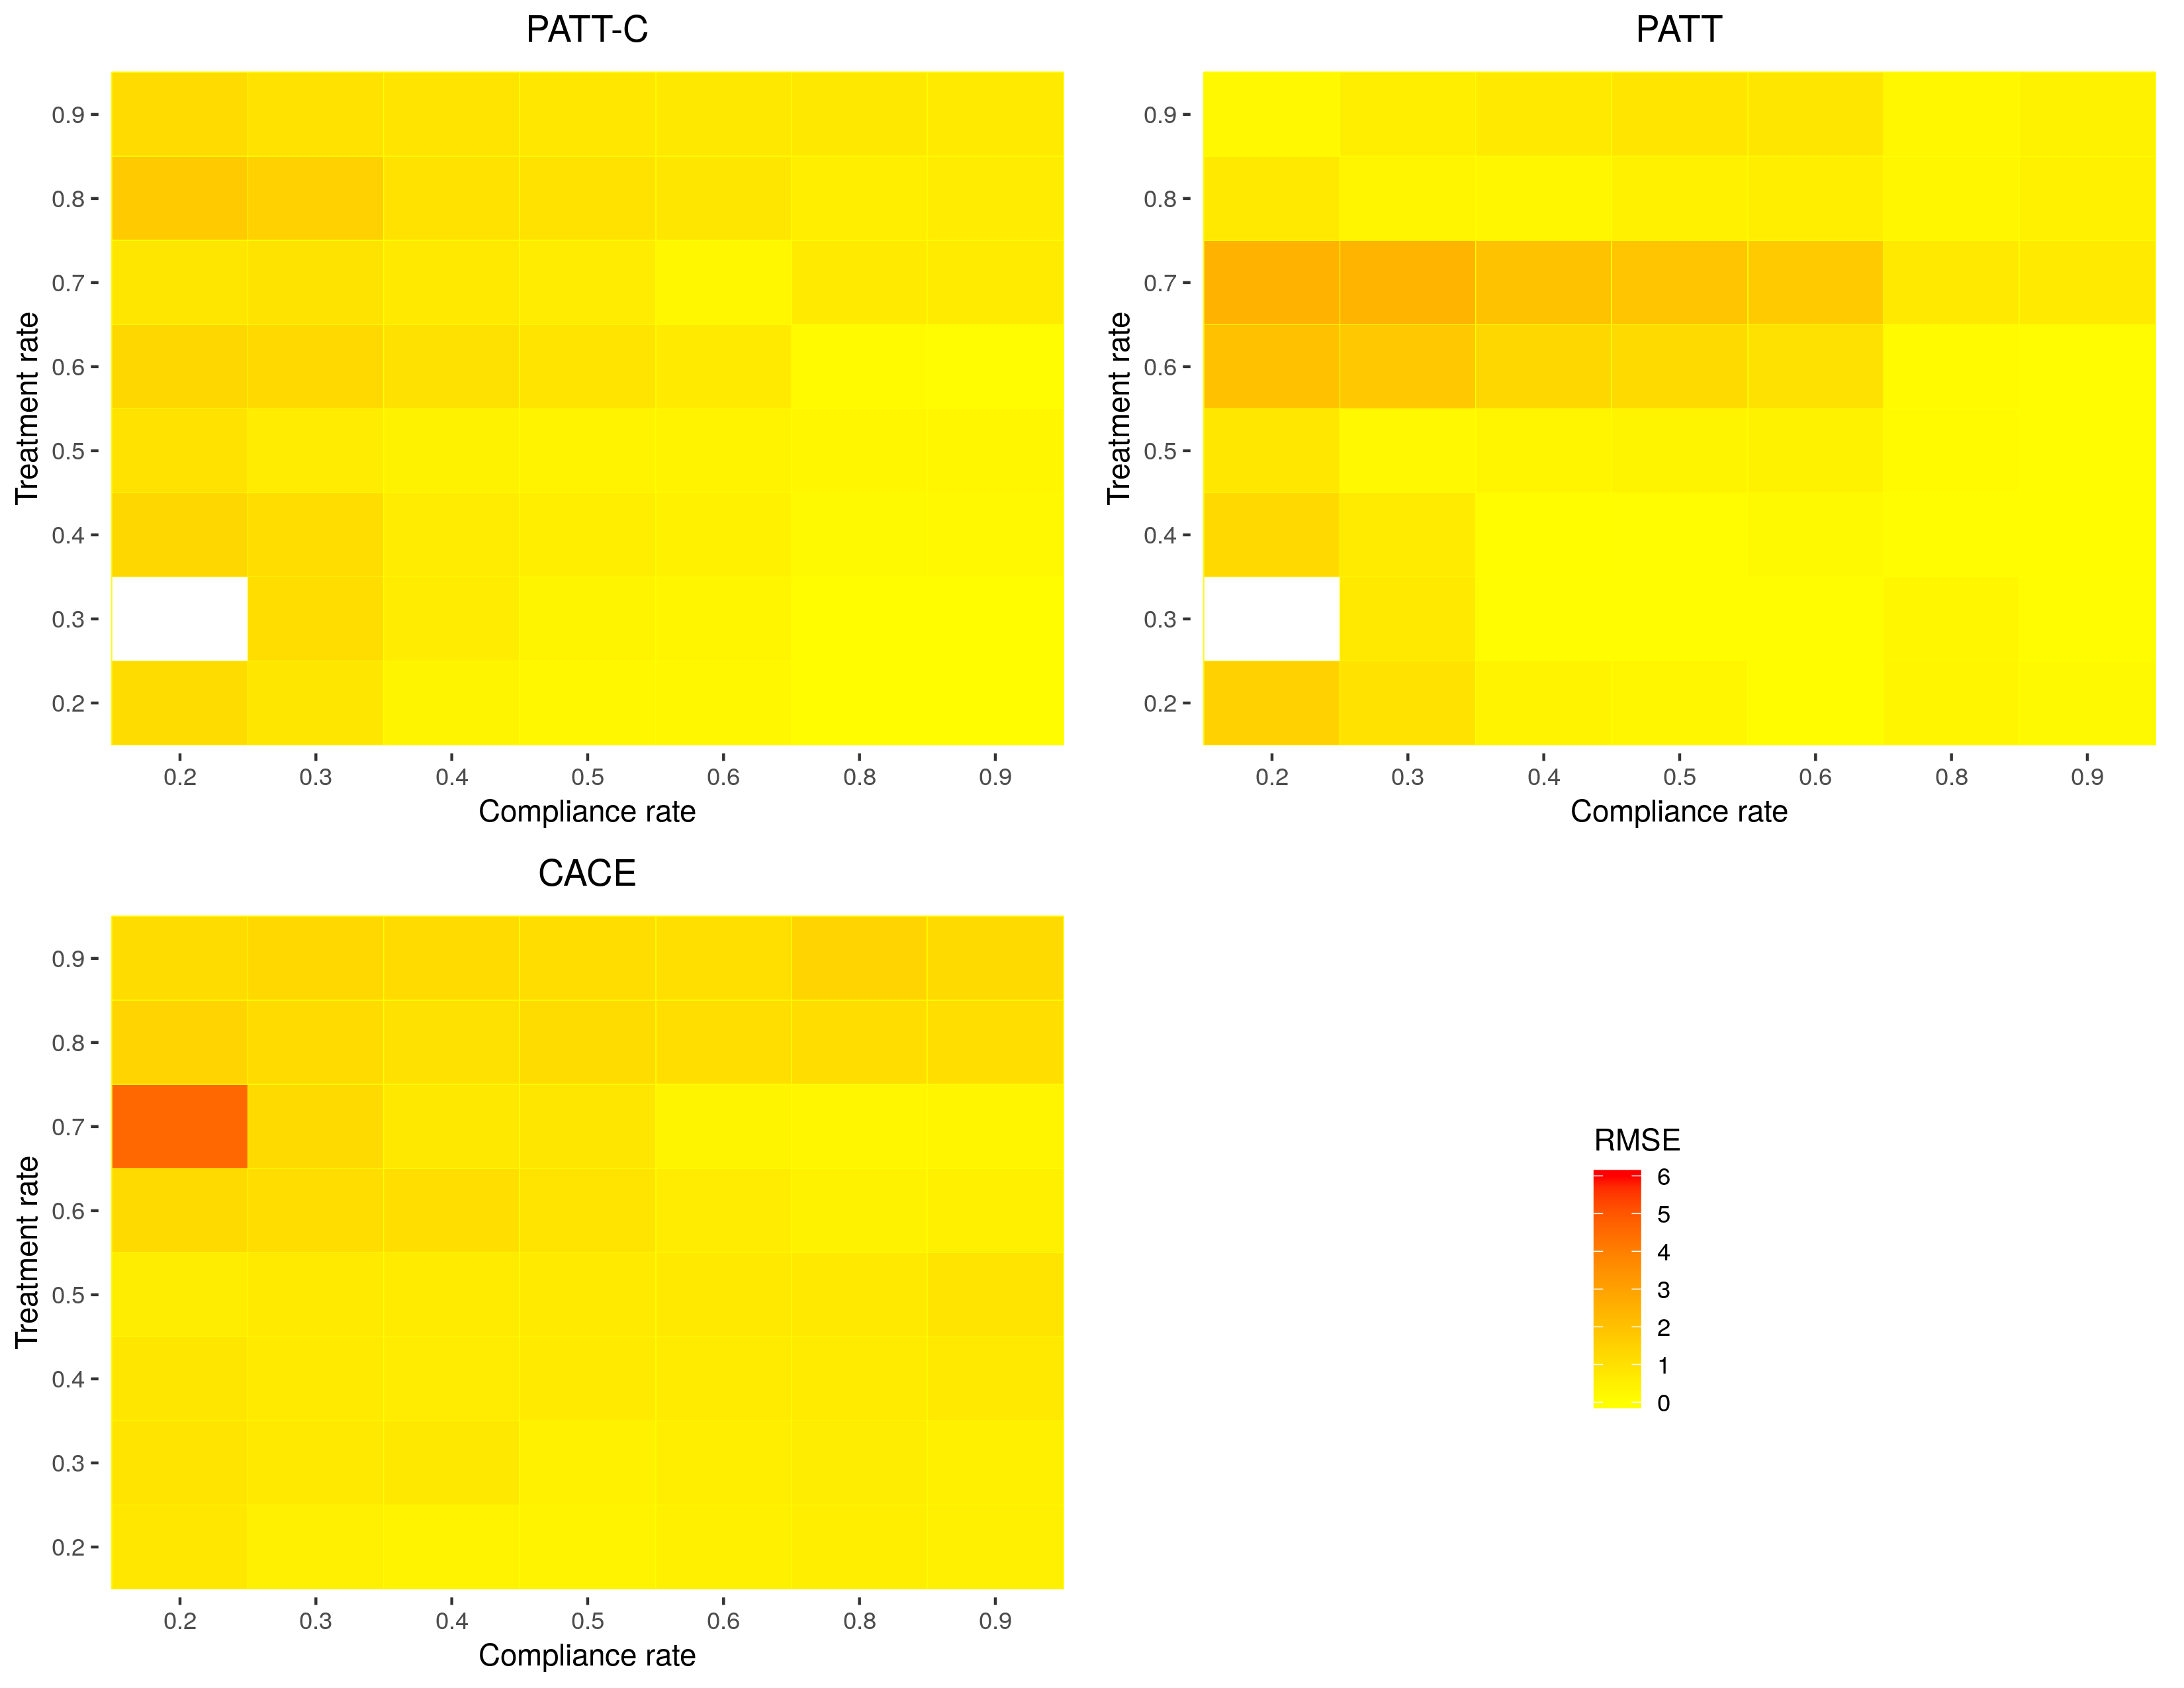
\includegraphics[width = 1\textwidth]{rmse_ratec_ratet}
		\caption{Simulated RMSE, binned by compliance rate and percent eligible for treatment. \label{fig:rmse_ratec_ratet}}
		%\caption{\label{fig:rmse_ratec_ratet}}
	\end{center}
\end{figure}

Figure~\ref{fig:sim_compliance} compares the RMSE of PATT and PATT-C with the SATT-C  at varying levels of compliance in the total population. When compliance is low, both PATT and PATT-C estimators have a large RMSE. The adjusted estimator has a large variance because the subset of the RCT who are considered compliers is relatively small, whereas the unadjusted estimator has bias from the large amount of crossover. For low levels of compliance, the SATT-C actually tends to estimate the average causal effects for the target population more closely than either PATT or PATT-C. On the other hand, when the compliance rate is high, both PATT and PATT-C estimators have low RMSE, with {\color{red} the} adjusted estimator performing slightly better. Meanwhile, the median RMSE for the SATT-C stays relatively constant regardless of compliance rate {\color{red}, and} the estimator is unbiased for the SATT-C rather than the PATT-C. The SATT-C estimate accounts for noncompliance, but is unable to account for differences in pretreatment covariates between the RCT sample and target population. This shows that {\color{red}reweighting or response surface methods} are needed to extrapolate RCT results to a wider population.

%
%\vspace{10mm}
%\begin{center}
%[FIGURE 3 HERE]
%\end{center}

\begin{figure}[htbp]
\begin{center}
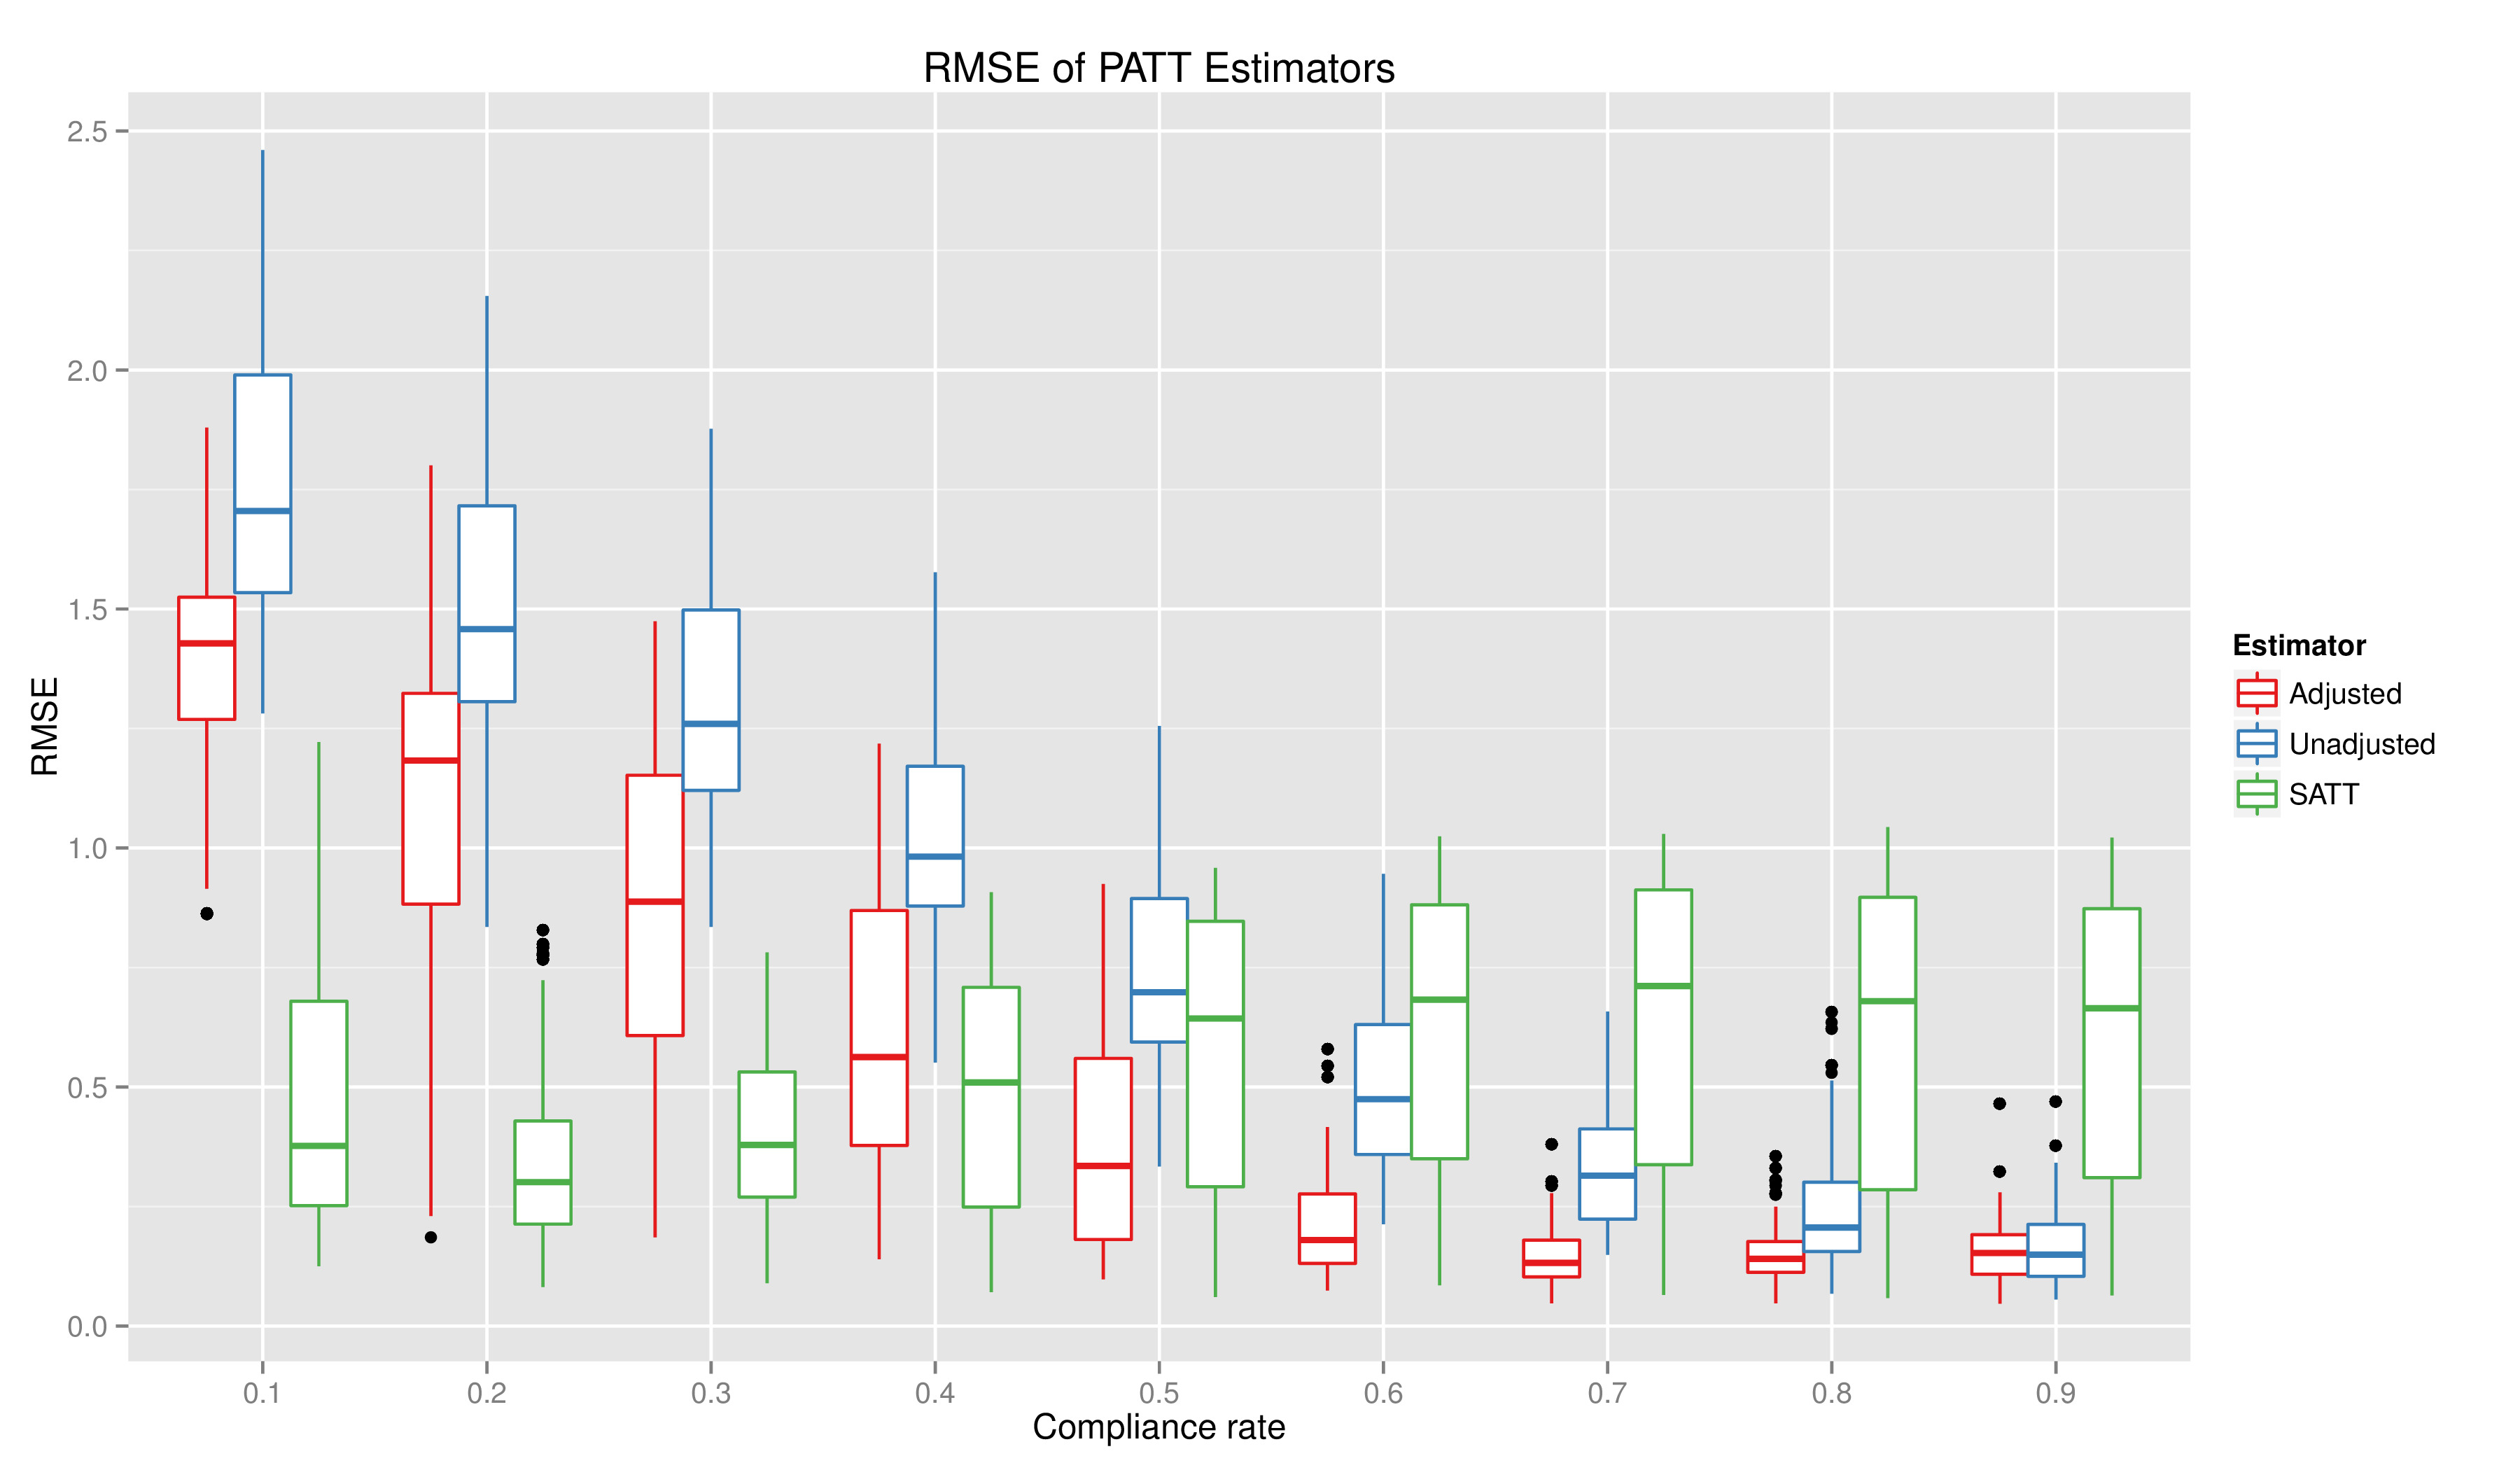
\includegraphics[width = 1\textwidth]{rmse_boxplots}
\caption{Simulated RMSE of PATT-C, PATT, and SATT-C, according to compliance rates in the total population.\label{fig:sim_compliance}}
%\caption{\label{fig:sim_compliance}}
\end{center}
\end{figure}

\section{Application: Medicaid and health care use} \label{application}

We apply the proposed estimator to measure the effect of Medicaid coverage on health care use for a target population of adults who may benefit from expansions to the Medicaid program. In particular, we examine the population of nonelderly adults in the U.S. with household incomes at or below 138\% of the Federal Poverty Level (FPL) --- which amounts to \$32,913 for a four--person household in 2014 --- who may be eligible for Medicaid following the Affordable Care Act (ACA) expansion.

\subsection{RCT sample} 

We draw RCT data from the Oregon Health Insurance Experiment (OHIE) \citep{finkelstein2012,baicker2013,baicker2014,Taubman}. In 2008, approximately 90,000 uninsured low-income adults participated in the OHIE to receive Medicaid benefits.\footnote{Eligible participants include Oregon residents (US citizens or legal immigrants) aged 19 to 64 not otherwise eligible for public insurance, who have been without insurance for six months, and have income below the FPL and assets below \$2,000.} Treatment occurred at the household level: participants selected by the lottery won the opportunity for themselves and any household member to apply for Medicaid. Within a sample of 74,922 individuals representing 66,385 households, 29,834 participants were selected by the lottery; the remaining 45,008 participants served as controls in the experiment. Participants in selected households received benefits if they returned an enrollment application within 45 days of receipt. Among participants in selected households, about 60\% mailed back applications and only 30\% successfully enrolled.\footnote{{\color{red}About half of the returned applications were deemed ineligible, primarily due to failure to demonstrate income below the FPL. Enrolled participants were required to recertify their eligibility status every six months.}}

The response data originate from a mail survey that was administered to participants over July and August 2009 ($n = 23,741$ survey respondents). We use the same definition of insurance coverage as \citet{finkelstein2012} to form our measure of compliance, which is a binary variable indicating whether the participant was enrolled in any Medicaid program between the notification date and 30 September 2009. The OHIE data include pretreatment covariates for gender, age, race, ethnicity, health status, education, and household income.

Our outcomes of interest are binary variables for any emergency room (ER) and outpatient visits in the past 12 months. {\color{red}ER use is an important outcome because it is the main delivery system through which the the uninsured receive health care. The uninsured could potentially receive higher quality and less affordable healthcare through outpatient visits. An important question for policymakers is whether Medicaid expansions will decrease ER utilization by the previously uninsured.   	

Subsequent research calls in to question the external validity of the OHIE, which resulted in the counterintuitive finding that Medicaid increased ER use among RCT participants \citep{finkelstein2012,Taubman}. For example, quasi-experimental studies on the impact of the 2006 Massachusetts health reform --- which served as a model for the ACA --- show that ER use decreased or remained constant following the reform \citep{miller2012effect, kolstad2012impact}. A challenge to the external validity of the OHIE is that it's exclusion criteria was likely more restrictive than government health insurance expansions. 
}

\subsection{Observational data} 

We acquire data on the target population from the National Health Interview Study (NHIS) for years 2008 to 2017 \citep{NHIS}.\footnote{{\color{red}A possible limitation of this application is that it ignores the complex sampling techniques of the NHIS sample design such as differential sampling, which is discussed in detail in \citet{parsons2014design}.}\label{nhis-ftn}} We restrict our sample to respondents with income below 138\% of the FPL and who are uninsured or on Medicaid ($n=11,129$). We select covariates on respondent characteristics that match the OHIE pretreatment covariates. The outcomes of interest from NHIS are variables on ER and outpatient visits in the past 12 months. We use a recoded variable that indicates whether respondents are on Medicaid as an analogue to the OHIE compliance measure. 

\subsection{Verifying assumptions} \label{verifying}

In order for $\tau_{\text{PATT-C}}$ to be identified, Assumptions \ref{consistency} -- \ref{ER} must be met. Assumption \ref{consistency} ensures that potential outcomes for participants in the target population (i.e., respondents in the NHIS sample) would be identical to their outcomes in the RCT if they had been randomly assigned their observed treatment. {\color{red}Medicaid coverage for uninsured individuals was applied in the same manner in the RCT as it is in the population.  Differences in potential outcomes due to sample selection might arise, however, if there are differences in the mail surveys used to elicit health care use responses between the RCT and the nonrandomized study. }
 
We cannot directly test Assumptions \ref{si_treat} and \ref{si_ctrl}, which state that potential outcomes for treatment and control are independent of sample assignment for individuals with the same covariates and assignment to treatment. The assumptions are only met if every possible confounder associated with the response and the sample assignment is accounted for. In our estimation of the response surface, we use all demographic, socioeconomic, and pre-existing health condition data that were common in the OHIE and NHIS data. Potentially important unobserved confounders include the number of hospital and outpatient visits in the previous year, proximity to health services, and enrollment in other federal programs. 

Table~\ref{rct-nrt-compare} compares RCT participants selected for Medicaid with NRT participants on Medicaid. Compared to the RCT treated, the target population ``treated''  group is predominantly female, younger, more racially and ethnically diverse, less educated, and live in higher income households. Diagnoses of diabetes, asthma, high blood pressure, and heart disease are more common among the population on Medicaid then the RCT treated.

\newgeometry{left=3cm,bottom=0.1cm}
\begin{singlespace}
\begin{longtable}{lllllll}
\caption{Pretreatment covariates and responses for OHIE and NHIS respondents on Medicaid.\label{rct-nrt-compare}} \\
  & OHIE &  & OHIE &  & NHIS &  \\ 
    & control &  & treated &  &treated &   \\ 
  & $n=5,476$ &  & $n=5,193$ &  & $n=3,382$ &  \\  
  \hline   
    \hline   
 \textbf{Covariate} &  $\mathbf{n}$ & $\mathbf{\%}$ & $\mathbf{n}$ & $\mathbf{\%}$ & $\mathbf{n}$ & $\mathbf{\%}$ \\ 
\hline
\textit{Sex:} &  & & &  &  & \\ 

\hspace{3mm} Female & 3,148 & 57.5 & 2,920 & 56.2 & 2,380 & 70.4 \\ 
 &  & & &  &  & \\ 
\textit{Age:} &  & & &  &  & \\ 
\hspace{3mm}19-49 & 1,636 & 29.9 & 1,367 & 26.3 & 2,429 & 71.8  \\ 

\hspace{3mm}50-64 & 3,840 & 70.1 & 3,826 & 73.7 & 953 & 28.2 \\ 
 &  & & &  &  & \\ 
\textit{Race:} &  & & &  &  & \\ 
\hspace{3mm}White & 4,829 & 88.2 & 4,393 & 84.6 & 1,991 & 58.9  \\ 

\hspace{3mm}Black & 243 & 4.4 & 197 & 3.8 & 1,050 & 31.1  \\ 

\hspace{3mm}Hispanic & 301 & 5.5 & 476 & 9.2 & 910 & 26.9  \\ 
 &  & & &  &  & \\ 
\textit{Health status:} &  & & &  &  & \\ 
\hspace{3mm}Diabetes & 581 & 10.6 & 539 & 10.4 & 452 & 13.4 \\ 

\hspace{3mm}Asthma & 1,036 & 18.9 & 887 & 17.1 & 652 & 19.3  \\ 

\hspace{3mm}High blood pressure & 1,670 & 30.5 & 1,418 & 27.3 & 1,143 & 33.8  \\ 
  
\hspace{3mm}Heart condition & 170 & 3.1 & 141 & 2.7 & 285 & 8.4 \\ 
 &  & & &  &  & \\ 
\textit{Education:} &  & & &  &  & \\  
\hspace{3mm}Less than high school  & 1,056 & 19.3 & 950 & 18.3 & 1,183 & 35.0  \\ 
  
\hspace{3mm}High school diploma or GED & 3,081 & 56.3 & 2,775 & 53.4 & 1,076 & 31.8  \\ 

\hspace{3mm}Voc. training / 2-year degree & 969 & 17.7 & 1,031 & 19.9 & 934 & 27.6 \\ 

\hspace{3mm}4-year college degree or more & 370 & 6.8 & 437 & 8.4 & 189 & 5.6 \\ 
 &  & & &  &  & \\ 
\textit{Income:} &  & & &  &  & \\ 
\hspace{3mm} $<\$10$k & 5,476 & 100.0 & 3,204 & 61.7 & 1,452 & 42.9 \\

\hspace{3mm} \$10k-\$25k & 0 & 0.0 & 1,616 & 31.1 & 1,622 & 48.0 \\

\hspace{3mm} $>\$25$k & 0 & 0.0 & 373 & 7.2 & 308 & 9.1 \\
   \hline
\hline
 \textbf{Response} &   &  &  & &  &  \\ 
\hspace{3mm}Any ER visit &  1,393 & 25.4 & 1,301 & 25.1 & 881 & 26.1 \\ 
\hspace{3mm}Any outpatient visit & 3,299 & 60.2 & 3,081 & 59.3 & 2,116 & 62.6 \\ 
\hline
\hline
\end{longtable}
\end{singlespace}
\restoregeometry

{\color{red}Strong ignorability assumptions may also be violated due to the fact that the OHIE applied a more stringent exclusion criteria compared to the NHIS sample. While the RCT and population sample both screened for individuals below the FPL, only the RCT required those enrolled to recertify their eligibility status every six months.}

A violation of the assumption of no-interference (Assumption \ref{sutva}) biases the estimate of $\tau_{\text{PATT-C}}$ if, for instance, treated participants' Medicaid coverage makes control participants more likely to visit the ER. Interference is less likely in this experimental set--up because treatment occurs at the household level. Assumption \ref{compl} is violated if assignment to treatment influences the compliance status of individuals with the same covariates. Our compliance model can accurately classify compliance status for 77\% of treated RCT participants with only the covariates --- and not treatment assignment --- as features.\footnote{The 10--fold cross--validated risk estimate on the training set is 22.6\%. Information on the ensemble's candidate algorithms and corresponding risk estimates are provided in Table \ref{compliance-ensemble}.}  This gives evidence in favor of the conditional independence assumption.

The exclusion restriction (Assumption \ref{ER}) ensures treatment assignment affects the response only through enrollment in Medicaid. It is reasonable that a person's enrollment in Medicaid, not just their eligibility to enroll, would affect their hospital use. For private health insurance one might argue that eligibility may be be negatively correlated with hospital use, as people with pre-existing conditions are less often eligible yet go to the hospital more frequently. This should not be the case with a federally funded program such as Medicaid. 

{\color{red}
\subsubsection{Sensitivity to no defiers assumption} \label{sens-defiers}
}

\citet{Angrist1996} show that the bias due to violations of Assumption \ref{monotonicity} is equivalent to the difference of average causal effects of treatment received for compliers and defiers, multiplied by the relative proportion of defiers, 
$\pr(i\text{ is a defier}) / (\pr(i\text{ is a complier]}) - \pr(i\text{ is a defier})).$

Table \ref{ohie-status} reports the distribution of participants in the OHIE by status of treatment assignment and treatment received. Assumption \ref{monotonicity} does not hold due to the presence of defiers; i.e., participants who were assigned to control and enrolled in Medicaid during the study period. About 6.7\% of the RCT sample were assigned to control but were enrolled in Medicaid ($T_i < D_i$) and 65.5\% of the sample complied with treatment assignment ($D_i = T_i$), which results in a bias multiplier of 0.11. Suppose that the difference of average causal effects of Medicaid received on ER use for compliers and defiers is 1.2\%.\footnote{This quantity is the difference between the adjusted and unadjusted SATT on ER use reported in Section \ref{results}.} The resulting bias is only 0.1\%, which would not meaningfully alter the interpretation of the SATT-C or PATT-C reported in Section \ref{results}. 
 
\subsection{Empirical results}\label{results}

We compare PATT-C and SATT estimates for ER and outpatient use. We obtain estimates for the overall group of participants and subgroups according to sex, age, race, health status, education, and household income. Subgroup treatment effects are estimated by taking differences across response surfaces for a given covariate subgroup, and response surfaces are estimated with random forests.\footnote{The 10--fold cross-validated risk estimate of the random forests model (default settings) range from 0.24 to 0.331.} We use treatment assignment, number of household members, and the subgroup covariates as features in the response models. We generate 95\% confidence intervals for these estimates using 1,000 bootstrap samples.% The entire RCT sample size is $n=23,205$ and the population sample is $n=11,129$. There are $n=10,669$ RCT compliers and $n=3,382$ target population ``compliers'' on Medicaid. 

Figure \ref{fig:any-visit-plot} compares treatment effect estimates on ER use. We estimate the effect of Medicaid coverage on the likelihood of visiting the ER is about 1.3\% for population compliers (PATT-C). In comparison, the effect on RCT compliers (SATT-C) is 1.2\% and RCT participants assigned to treatment (SATT) is about zero. There are substantial differences between sample and population estimates across covariate groups. For instance, the treatment effect on ER use for white sample participants is positive, but negative for white population participants. Treatment effects on ER use tend to be large and significant for RCT participants with health conditions, but negative for the corresponding population participants.
%
%\vspace{10mm}
%\begin{center}
%[FIGURE 4 HERE]
%\end{center}

\begin{figure}[htbp]
\begin{center}
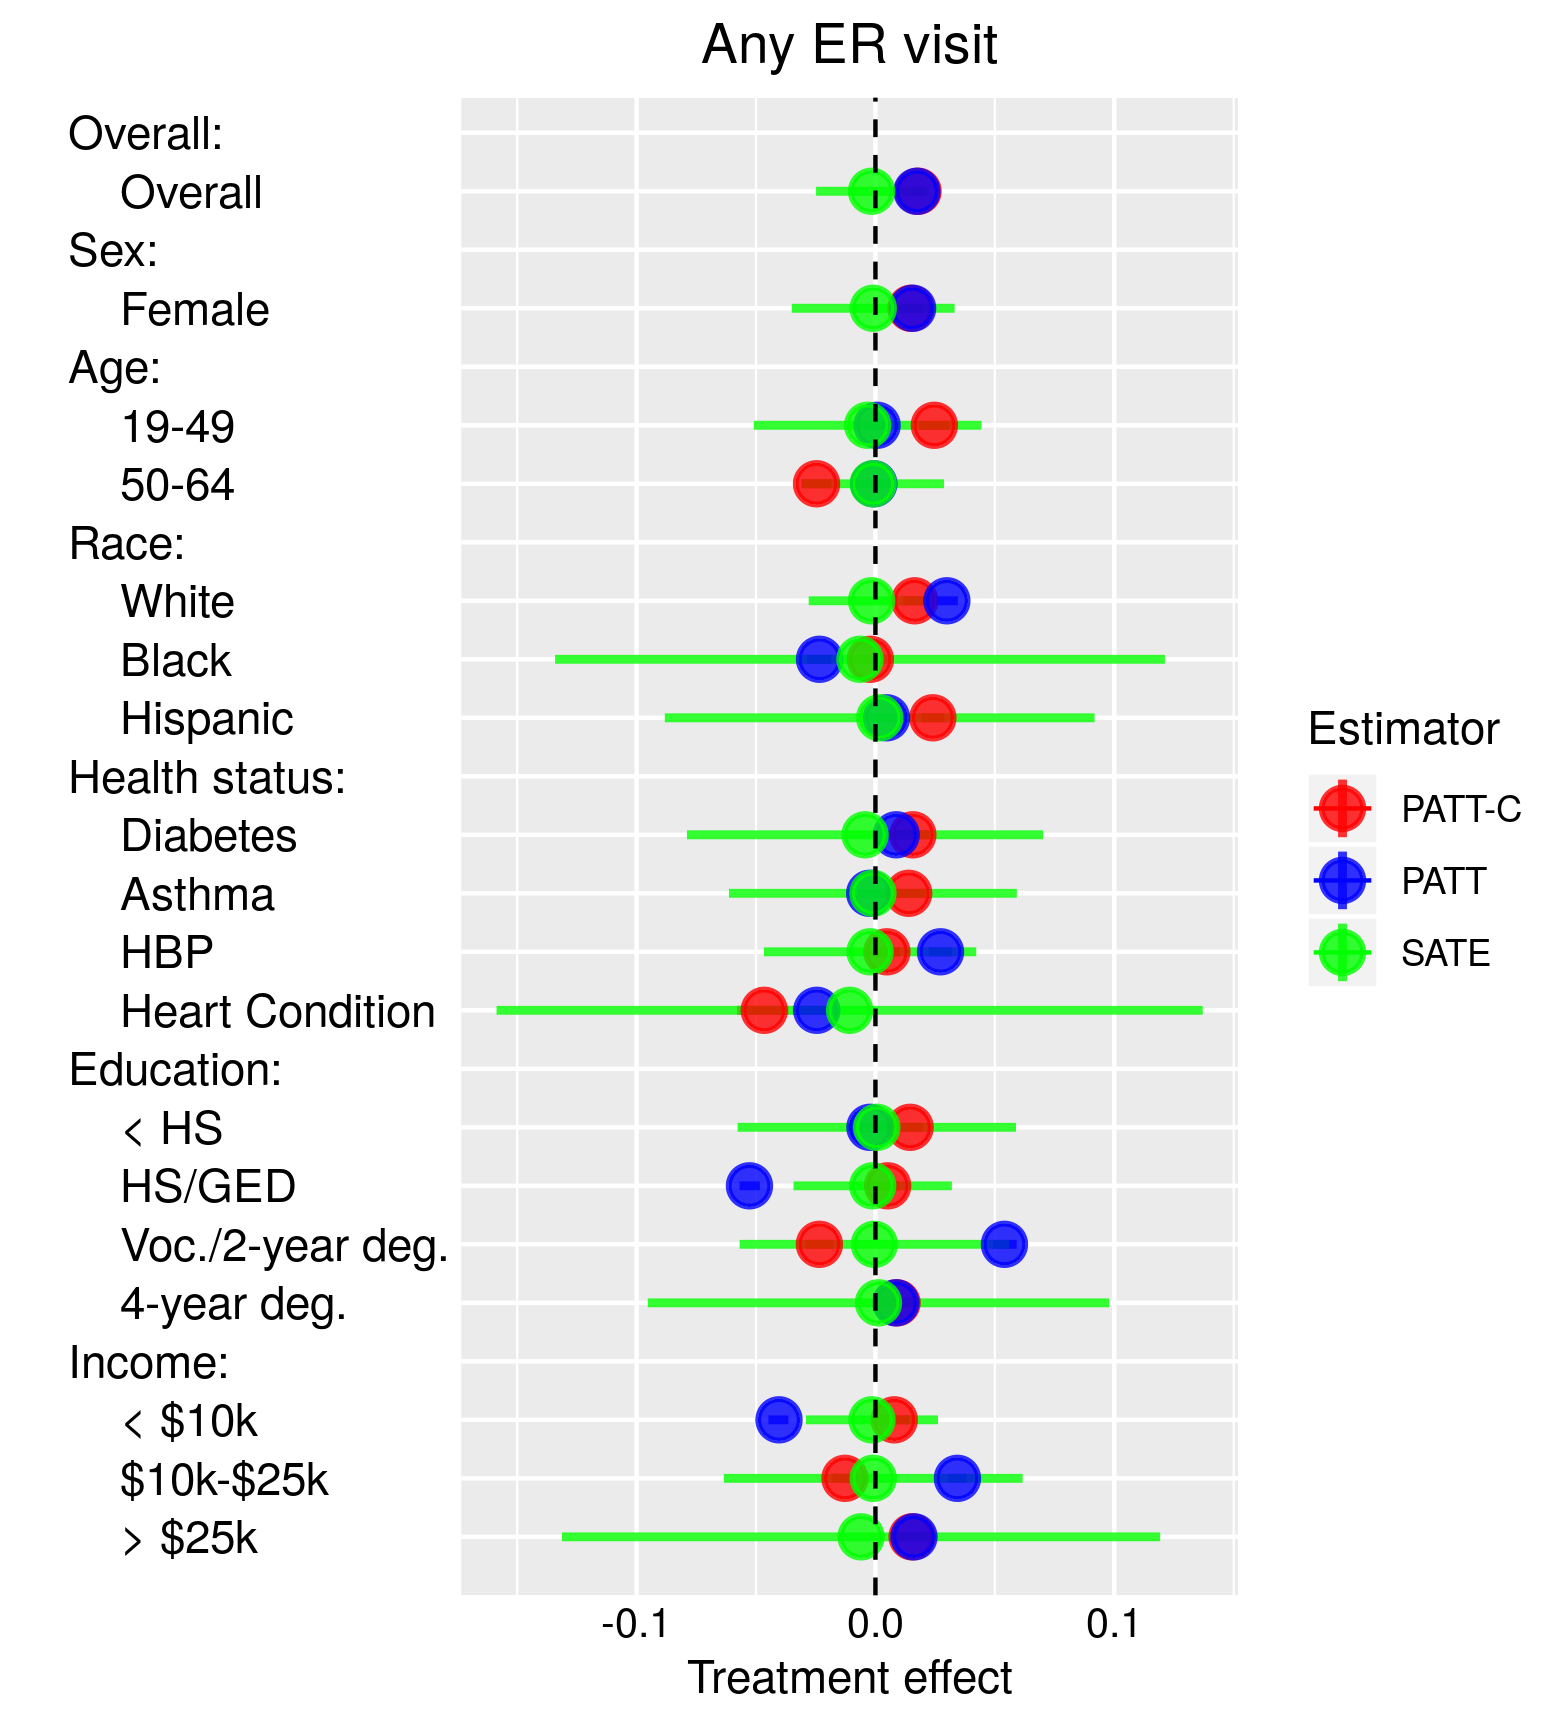
\includegraphics[width = 0.9\textwidth]{any-visit-plot}
    \caption{Comparison of estimators: any ER visit. Horizontal lines represent 95\% bootstrap confidence intervals.\label{fig:any-visit-plot}}
%\caption{\label{fig:any-visit-plot}}
\end{center}
\end{figure}

Figure \ref{fig:any-out-plot} compares treatment effect estimates on outpatient use. For population compliers, the effect of Medicaid coverage on the likelihood of outpatient use is -2.5\%. In comparison, the effect is -2\% for RCT compliers and -1.2\% for RCT participants assigned to treatment. Treatment effects on outpatient use are large and positive for college--educated RCT compliers, but about zero for college--education population compliers. 
%
%\vspace{15mm}
%\begin{center}
%[FIGURE 5 HERE]
%\end{center}

\begin{figure}[htbp]
\begin{center}
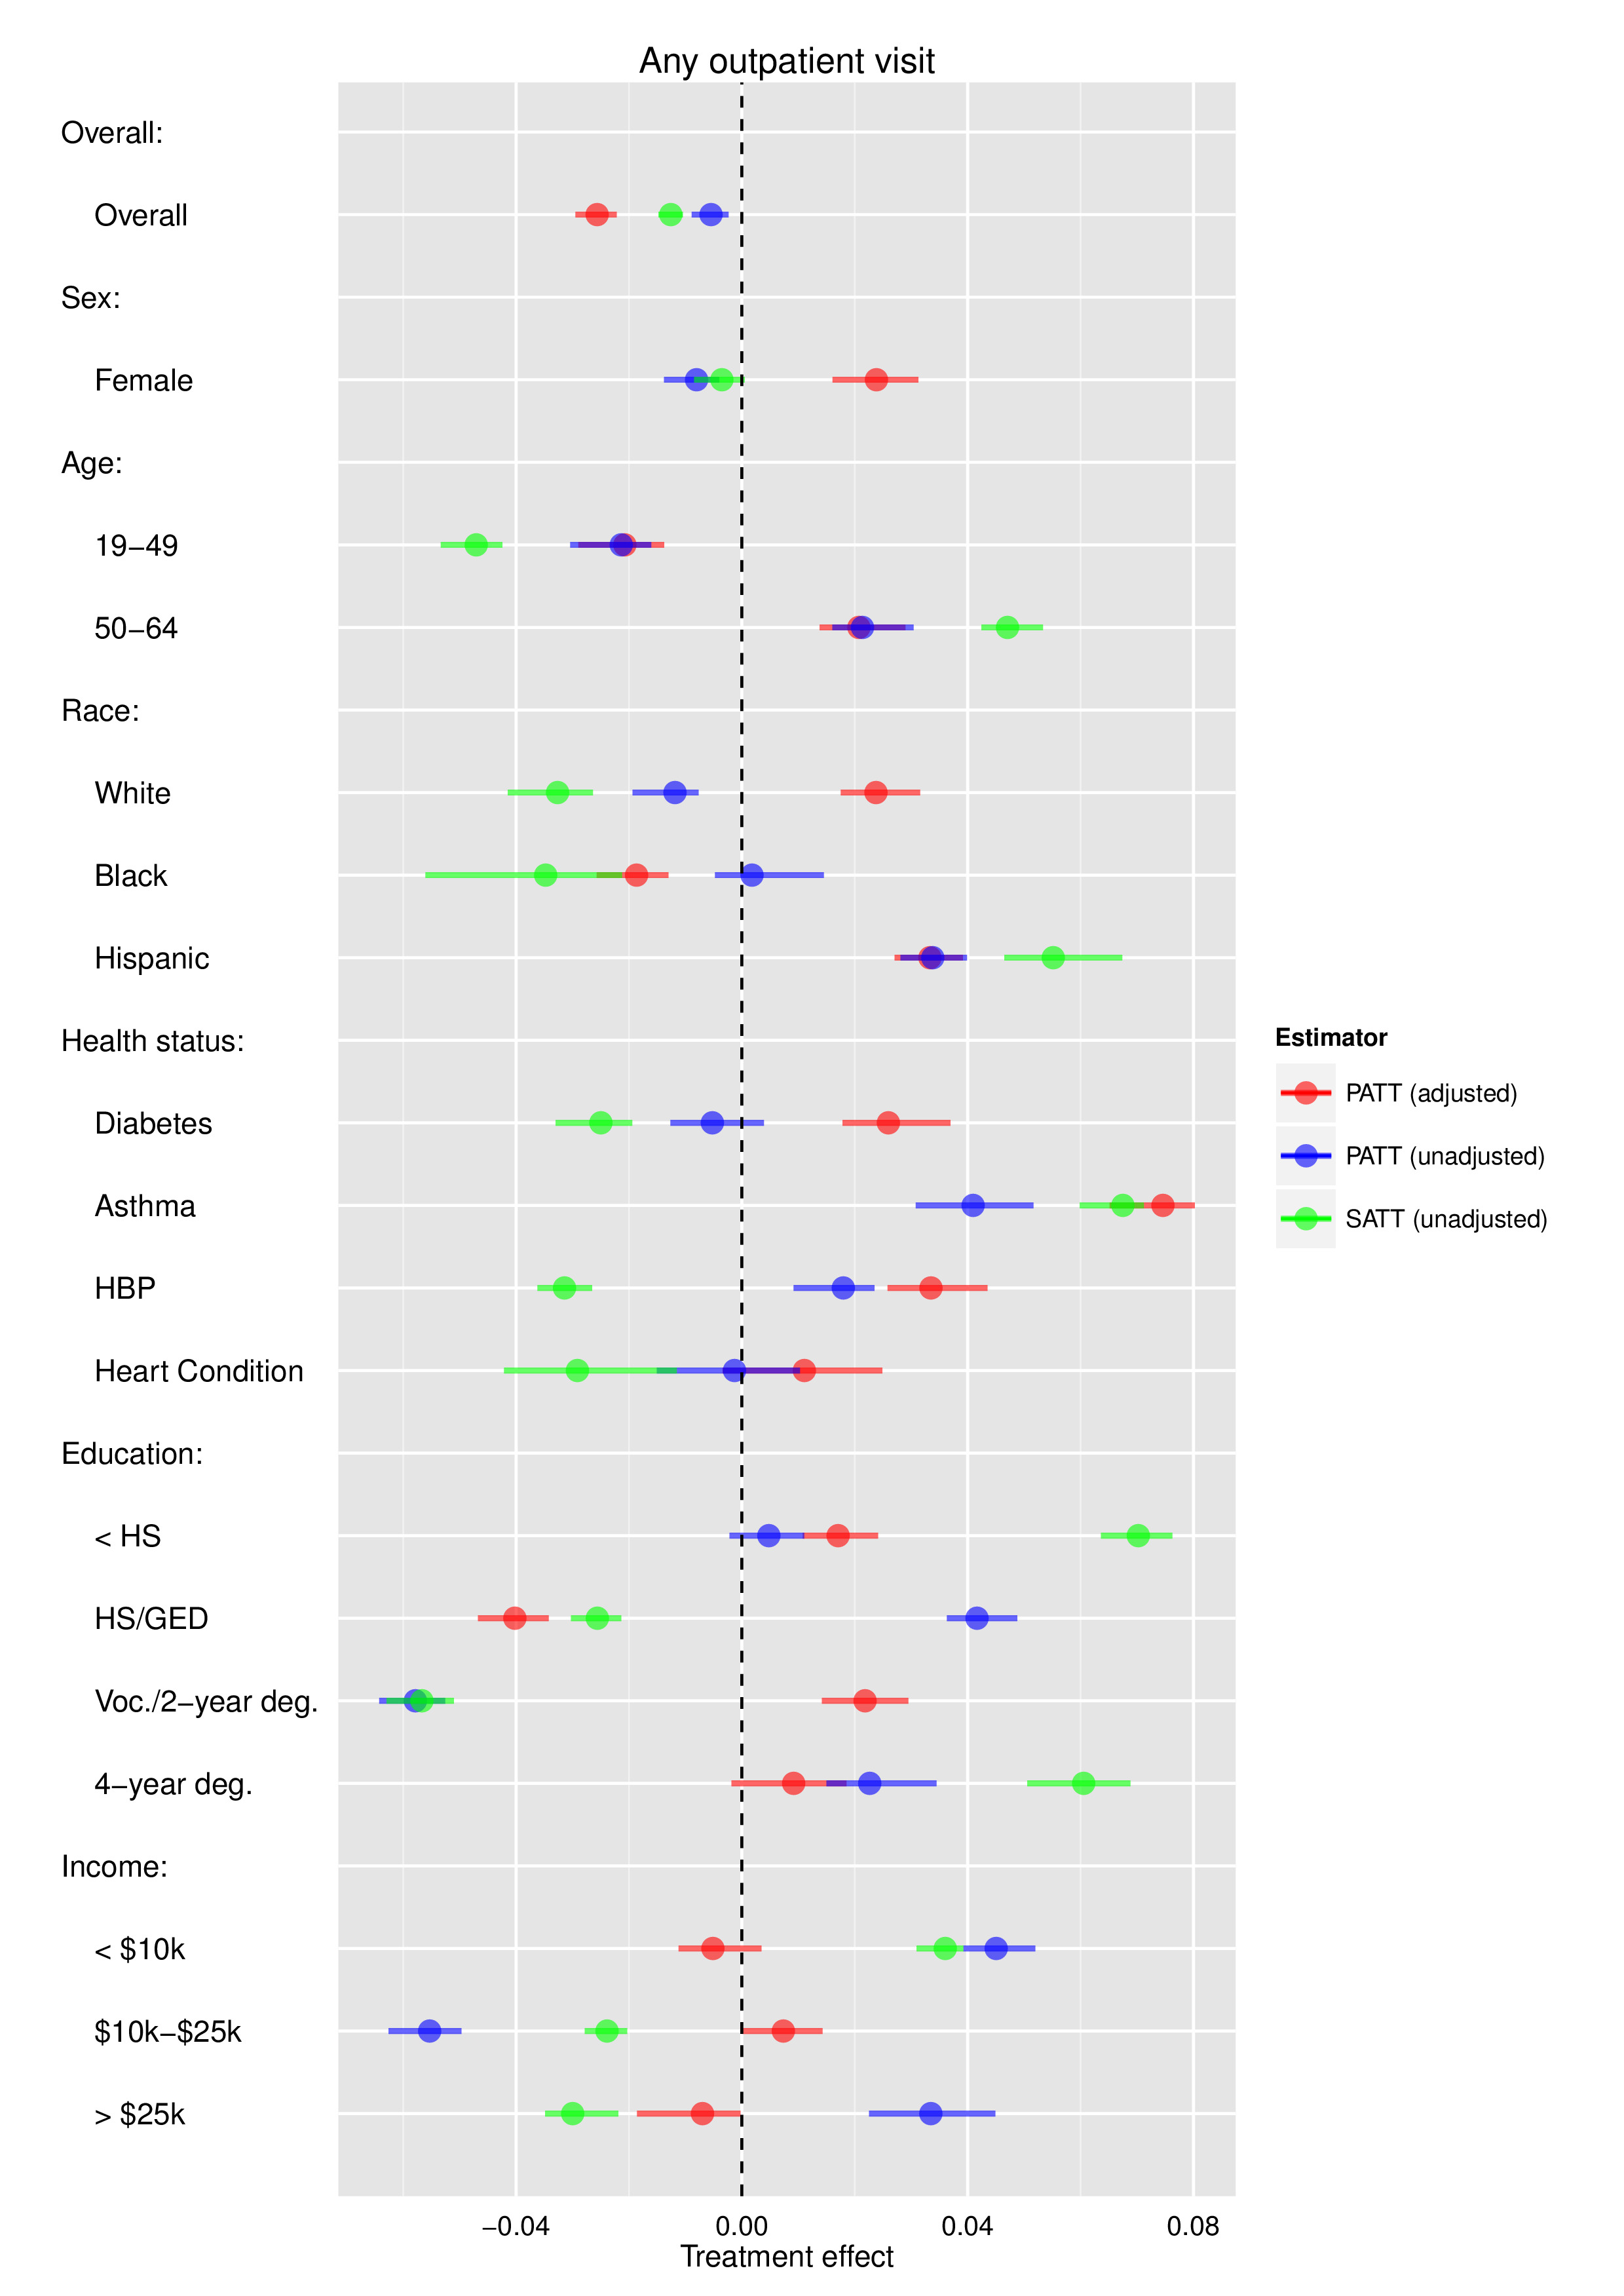
\includegraphics[width = 0.9\textwidth]{any-out-plot}
    \caption{Comparison of estimators: any outpatient visit. Horizontal lines represent 95\% bootstrap confidence intervals.\label{fig:any-out-plot}}
%\vspace{10mm}
%\caption{\label{fig:any-out-plot}}
%\vspace{10mm}
\end{center}
\end{figure}

{\color{red}
\subsubsection{Comparison with previous results} \label{results-compare}
}
We compare our population estimates with \citet{finkelstein2012}, who report population estimates of the effect of Medicaid coverage on \emph{the number of} ER and out-patient visits using 2004--2009 NHIS data on adults aged 19--64 below 100 percent of the federal poverty line ($n=15,528$). Similar to our PATT-C estimates on the likelihood of ER visits, \citet{finkelstein2012} estimates Medicaid coverage significantly increases the number of ER visits by 0.08 [0.05, 0.12]. While our PATT-C estimates indicate that Medicaid coverage decreases the likelihood of outpatient visits, the authors estimate Medicaid increases the number of outpatient visits in the NHIS sample by 1.45 [1.33, 1.57]. 

While our study is the first to our knowledge to estimate heterogeniety in treatment effects for the broader population, \citet{Taubman} and \citet{NBERw22363} perform subgroup analyses on the RCT sample. Across subgroups in the sample, \citet{Taubman} estimates mostly positive effects of Medicaid on ER use. Similar to our SATT-C estimates, \possessivecite{Taubman} subgroup analyses indicate that increases in ER use due to Medicaid are significantly larger for men and younger individuals in the sample. The authors also find that the effect of Medicaid on ER usage is larger for smokers. Individuals with an education level of high school and those pre-lottery diagnoses experience larger increases in ER use due to Medicaid, but these comparisons are not significant. \citet{NBERw22363} perform subgroup analyses on OHIE sample data and find larger increases in ER use as a result of Medicaid for men, English speakers, and individuals enrolled in a food stamp program prior to the lottery. 

\section{Discussion} \label{discussion}

The simulations presented in Section \ref{sim} shed light on the conditions under which the proposed estimator should work well. When the rate of crossover from treatment to control is low, the proposed estimator performs better than the estimator which doesn't adjust for noncompliance. Here, the unadjusted estimator gives the ITT effect, which tends to underestimate the average treatment effect on compliers. Of course, the simulation results depend on the particular way we parameterized the compliance, selection, treatment assignment, and response schedules. In particular, the strength of correlation between the covariates and compliance governs how well the estimator will perform, since \ref{compliance-model} of the estimation procedure is to predict who \textit{would be} a complier in the RCT control group, had they been assigned to treatment. If it is difficult to predict compliance using the observed covariates, then the estimator will perform badly because of noise introduced by incorrectly treating noncompliers as compliers. Further research should be done into ways to test how well the model of compliance works in the population. 

The proposed estimator, adjusting for noncompliance, performs better in simulations than the unadjusted estimator when compliance is low and can be predicted by observed covariates (Figure~\ref{fig:sim_compliance}). In the OHIE trial, only about $30\%$ of those selected to receive Medicaid benefits actually enrolled. Our ensemble method for predicting compliance based on observed covariates has $77\%$ accuracy on the training set of participants in the OHIE assigned to treatment. While we don't know how well the compliance model predicts for the control group, the control group should be similar to the treatment group on pretreatment covariates because of the randomization done. The model's performance on the training set suggests that compliance is not purely random and depends on observed covariates. This gives evidence in favor of using the proposed estimator. 

The treatment effect of Medicaid applies to uninsured adults with income below the FPL who express interest in health insurance coverage. The sample population differs in several dimensions from the target population of individuals who will be covered by other Medicaid expansions, such as the ACA expansion to cover all adults up to 138\% of the FPL. For instance, the RCT participants are disproportionately white urban--dwellers \citep{Taubman}. The RCT participants volunteered for the study and therefore may be in poorer health compared to the target population. These differences in baseline covariates make {\color{red}reweighting or response surface methods} necessary to extend the RCT results to the population.

Explicitly modeling compliance allows us to decompose SATT-C and PATT-C estimates by subgroup according to pretreatment covariates common to both RCT and observational datasets{\color{red}; e.g, demographic variables, pre--existing conditions, and insurance coverage}. We find substantial differences between sample and population estimates in terms of race, education, and health status subgroups. This pattern is expected because RCT participants volunteered for the study and are predominately white and educated.

Further research might explore models to more accurately predict compliance in RCTs. Our compliance model accurately classified compliance status for 77\% of treated RCT participants using only the pretreatment covariates as features. Accurately predicting compliance is not only essential for yielding unbiased estimates of the average causal effects for target populations, it is also useful for researchers and policymakers to know which groups of individuals are unlikely to comply with treatment. 

\pagebreak

%Bibliography
\printbibliography


%Appendix
\pagebreak
\begin{appendices}
	
% Appendix numbering
\newcommand{\hbAppendixPrefix}{A}
%
\renewcommand{\thefigure}{\hbAppendixPrefix\arabic{figure}}
\setcounter{figure}{0}
\renewcommand{\thetable}{\hbAppendixPrefix\arabic{table}} 
\setcounter{table}{0}
\renewcommand{\theequation}{\hbAppendixPrefix\arabic{equation}} 
\setcounter{equation}{0}

\begin{table}[h]
	\begin{center}
	\caption{Distribution of OHIE participants by status of treatment assignment ($T_i$) and treatment received ($D_i$).\label{ohie-status}} 
	\begin{tabular}{@{}llll@{}}
		\toprule
		& $D_i = 0$ & $D_i = 1$ & n      \\ \midrule
		$T_i = 0$ & 10,010    & 1,556     & 11,566 \\
		$T_i = 1$ & 6,446     & 5,193     & 11,639 \\
		n         & 16,456    & 6,749     & 23,205 \\ \bottomrule
	\end{tabular}
	\end{center}
\end{table}

% complier-mod
\begin{table}[h]
\begin{center}
\caption{Error and weights for ensemble for compliance model.\label{compliance-ensemble}} 
\begin{tabular}{llcc}
  \hline
 Algorithm & Parameters & MSE & Weight \\ 
  \hline
%        \rowcolor{Gray}
Super learner (\texttt{SuperLearner}) & default & 0.22 &   \\
%Discrete SL & default & 0.226 0.001 0.222 0.231 \\
GBM (\texttt{gbm}) & default & 0.22 &  \\ 
Lasso regression (\texttt{glmnet})  & $\alpha=1$ & 0.22 &   \\ 
Regularized linear model (\texttt{glmnet}) &  $\alpha=0.25$ & 0.22 &   \\ 
Regularized linear model (\texttt{glmnet}) &  $\alpha=0.5$ & 0.22 &  \\ 
Regularized linear model (\texttt{glmnet}) &  $\alpha=0.75$ & 0.22 &  \\ 
Neural network (\texttt{nnet}) &  default & 0.227 &  \\ 
Random forests (\texttt{randomForest}) & default & 0.307 &    \\  
Random forests (\texttt{randomForest})  &  $\# \, \text{preds.} =1$ & 0.27 &  \\ 
Random forests (\texttt{randomForest})  &  $\# \, \text{preds.} =5$  & 0.30 &  \\  
Random forests (\texttt{randomForest})  &  $\# \, \text{preds.} =10$ & 0.31 &   \\ 
Ridge regression (\texttt{glmnet}) &  $\alpha=0$ & 0.227 &  \\ 
   \hline
\end{tabular} 
\end{center}
\footnotesize{{\color{red}Notes: cross-validated error and weights used for each algorithm in super learner prediction ensemble for record classification model. \textit{MSE} is the ten-fold cross-validated mean squared error for each algorithm. \textit{Weight} is the coefficient for the Super Learner, which is estimated using non-negative least squares based on the Lawson-Hanson algorithm. $\alpha$ is the elasticnet regularization parameter, where $\alpha = 0$ is the ridge penalty and $\alpha = 1$ is the lasso penalty. $\# \, \text{preds.}$ is the number of predictors sampled for splitting at each node.}}
\end{table}

\pagebreak
%\section{Ensemble method for response models} 

%\subsection{Response model on RCT compliers}

\begin{table}[h]
\caption{Error and weights for ensemble method for response model on RCT compliers.\label{reponse-ensemble}}  
  \begin{tabularx}{\linewidth}{l*{4}{Y}}
    \toprule
    \multicolumn{4}{l}{\textbf{Any ER visit}} \\
    \midrule
 Algorithm & Parameters & MSE & Weight \\ 
  \hline
GBM (\texttt{gbm}) & default & 0.18 & 0  \\ 
Lasso regression (\texttt{glmnet})  & $\alpha=1$& 0.18 & 1 \\ 
Regularized linear model (\texttt{glmnet}) &  $\alpha=0.25$ & 0.18 & 0 \\ 
Regularized linear model (\texttt{glmnet}) &  $\alpha=0.5$ & 0.18 & 0 \\ 
Regularized linear model (\texttt{glmnet}) &  $\alpha=0.75$ & 0.18 & 0 \\ 
Neural network (\texttt{nnet}) &  default & 0.234 & 0 \\ 
Random forests (\texttt{randomForest}) & default & 0.24 & 0 \\ 
Random forests (\texttt{randomForest})  & $\# \, \text{preds.} =1$ & 0.25 & 0 \\ 
Random forests (\texttt{randomForest})  & $\# \, \text{preds.} =5$  & 0.24 & 0 \\ 
Random forests (\texttt{randomForest})  & $\# \, \text{preds.} =10$ & 0.24 & 0 \\ 
Ridge regression (\texttt{glmnet}) &  $\alpha=0$ & 0.188 & 0 \\ 
   \hline
  \end{tabularx}
  \begin{tabularx}{\linewidth}{l*{4}{Y}}
    \toprule
    \multicolumn{4}{l}{\textbf{Any outpatient visit}} \\
    \midrule
Algorithm & Parameters & MSE & Weight \\ 
\hline
GBM (\texttt{gbm}) & default & 0.24 & 0  \\ 
Lasso regression (\texttt{glmnet})  & $\alpha=1$& 0.24 & 0 \\ 
Regularized linear model (\texttt{glmnet}) &  $\alpha=0.25$ & 0.24 & 0 \\ 
Regularized linear model (\texttt{glmnet}) &  $\alpha=0.5$ & 0.24 & 0.76 \\ 
Regularized linear model (\texttt{glmnet}) &  $\alpha=0.75$ & 0.24 & 0 \\ 
Neural network (\texttt{nnet}) &  default & 0.24 & 0 \\ 
        \rowcolor{Gray}
Random forests (\texttt{randomForest}) & default & 0.33 & 0 \\ 
Random forests (\texttt{randomForest})  & $\# \, \text{preds.} =1$ & 0.39 & 0.23 \\ 
Random forests (\texttt{randomForest})  & $\# \, \text{preds.} =5$  & 0.33 & 0 \\ 
Random forests (\texttt{randomForest})  & $\# \, \text{preds.} =10$ & 0.33 & 0.01 \\ 
Ridge regression (\texttt{glmnet}) &  $\alpha=0$ & 0.24 & 0 \\ 
   \hline
    \bottomrule
  \end{tabularx}
\footnotesize{See notes to Fig.\ref{compliance-ensemble}.}
\end{table}

\pagebreak
%\subsection{Response model on all RCT participants}

\begin{table}[ht]
\caption{Error and weights for ensemble method for response model on all RCT participants.\label{reponse-ensemble-unadj}}  
  \begin{tabularx}{\linewidth}{l*{4}{Y}}
    \toprule
    \multicolumn{4}{l}{\textbf{Any ER visit}} \\
    \midrule
 Algorithm & Parameters & MSE & Weight \\ 
  \hline
GBM (\texttt{gbm}) & default & 0.18 & 0  \\ 
Lasso regression (\texttt{glmnet})  & $\alpha=1$& 0.18 & 0.54 \\ 
Regularized linear model (\texttt{glmnet}) &  $\alpha=0.25$ & 0.18 & 0 \\ 
Regularized linear model (\texttt{glmnet}) &  $\alpha=0.5$ & 0.18 & 0 \\ 
Regularized linear model (\texttt{glmnet}) &  $\alpha=0.75$ & 0.18 & 0 \\ 
Neural network (\texttt{nnet}) &  default & 0.22 & 0 \\ 
Random forests (\texttt{randomForest}) & default & 0.24 & 0 \\ 
Random forests (\texttt{randomForest})  & $\# \, \text{preds.} =1$ & 0.25 & 0 \\ 
Random forests (\texttt{randomForest})  & $\# \, \text{preds.} =5$  & 0.24 & 0 \\ 
Random forests (\texttt{randomForest})  & $\# \, \text{preds.} =10$ & 0.24 & 0 \\ 
Ridge regression (\texttt{glmnet}) &  $\alpha=0$ & 0.18 & 0.45 \\ 
   \hline
  \end{tabularx}
  \begin{tabularx}{\linewidth}{l*{4}{Y}}
    \toprule
    \multicolumn{4}{l}{\textbf{Any outpatient visit}} \\
    \midrule
Algorithm & Parameters & MSE & Weight \\ 
\hline
GBM (\texttt{gbm}) & default & 0.23 & 0  \\ 
Lasso regression (\texttt{glmnet})  & $\alpha=1$& 0.23 & 0 \\ 
Regularized linear model (\texttt{glmnet}) &  $\alpha=0.25$ & 0.23 & 0 \\ 
Regularized linear model (\texttt{glmnet}) &  $\alpha=0.5$ & 0.23 & 0 \\ 
Regularized linear model (\texttt{glmnet}) &  $\alpha=0.75$ & 0.23 & 0 \\ 
Neural network (\texttt{nnet}) &  default & 0.24 & 0 \\ 
Random forests (\texttt{randomForest}) & default & 0.32 & 0 \\ 
Random forests (\texttt{randomForest})  & $\# \, \text{preds.} =1$ & 0.39 & 0.26 \\ 
Random forests (\texttt{randomForest})  & $\# \, \text{preds.} =5$  & 0.33 & 0 \\ 
Random forests (\texttt{randomForest})  & $\# \, \text{preds.} =10$ & 0.32 & 0.01 \\ 
Ridge regression (\texttt{glmnet}) &  $\alpha=0$ & 0.23 & 0.73 \\ 
   \hline
    \bottomrule
  \end{tabularx}
\footnotesize{See notes to Fig.\ref{compliance-ensemble}.}
\end{table}

\end{appendices}

\itemize
\end{document}


